% poglavlje_4.tex — Rezultati i analiza

\chapter{Rezultati i analiza}
\label{ch:rezultati}

\section{Eksperiment 1: Detekcija timing leaka}

\subsection{Deskriptivna statistika}

Cilj prvog eksperimenta je odgovoriti na osnovno pitanje: da li ranjiva square-and-multiply implementacija zaista ostavlja mjerljiv trag u trajanju operacije koji zavisi od vrijednosti tajnog bita? Eksperiment koristi paired dizajn opisan u sekciji \ref{sec:exp_design}, s ciljanim bitom na poziciji 16.

Nakon filtriranja rubnih vrijednosti (\textit{outlier}-a), mjerenja koja označavaju prekid od strane operativnog sistema, prikupljeno je ukupno 980\,050 validnih mjerenja za ranjivu implementaciju (odbačeno 2{,}0\%) i 980\,437 za constant-time implementaciju (odbačeno 2{,}0\%). Tabela \ref{tab:desc_stats} prikazuje deskriptivnu statistiku za obje implementacije.

\begin{table}[H]
\centering
\caption{Deskriptivna statistika trajanja modularne eksponencijacije (u CPU ciklusima)}
\label{tab:desc_stats}
\begin{tabular}{lrrr|rrr}
\toprule
 & \multicolumn{3}{c|}{\textbf{Ranjiva implementacija}} & \multicolumn{3}{c}{\textbf{Constant-time}} \\
\textbf{Metrika} & \textbf{bit=0} & \textbf{bit=1} & \textbf{$\Delta$} & \textbf{bit=0} & \textbf{bit=1} & \textbf{$\Delta$} \\
\midrule
$N$ uzoraka  & 490\,003  & 490\,047  & ---    & 490\,150  & 490\,287  & --- \\
Mean         & 8816{,}86 & 8892{,}77 & \textbf{+75{,}90} & 10689{,}68 & 10689{,}82 & $+$0{,}14 \\
Medijan     & 8824{,}00 & 8897{,}00 & \textbf{+73{,}00} & 10554{,}00 & 10554{,}00 & 0{,}00 \\
Std Dev      & 561{,}72  & 571{,}81  & +10{,}09  & 326{,}16  & 326{,}22  & $+$0{,}06 \\
P25          & 8406{,}00 & 8474{,}00 & \textbf{+68{,}00} & 10530{,}00 & 10530{,}00 & 0{,}00 \\
P75          & 9193{,}00 & 9275{,}00 & \textbf{+82{,}00} & 10619{,}00 & 10620{,}00 & $+$1{,}00 \\
\bottomrule
\end{tabular}
\end{table}

Rezultati za ranjivu implementaciju pokazuju jasnu i konzistentnu razliku između grupa bit=0 i bit=1. Prosječno trajanje operacije kada je tajni bit jednak 1 duže je za 75{,}90 CPU ciklusa u odnosu na slučaj kada je bit jednak 0. Ova razlika nije prisutna samo u aritmetičkoj sredini, već se proteže kroz sve mjere centralne tendencije: medijan pokazuje razliku od 73 ciklusa, donji kvartil (P25) 68 ciklusa, a gornji kvartil (P75) 82 ciklusa. Konzistentnost razlike na svim percentilima potvrđuje da se radi o pomjeranju cijele distribucije, a ne o slučajnosti koju bi mogle uzrokovati ekstremne vrijednosti.

Fizičko objašnjenje ove razlike je jasno: kada je bit eksponenta jednak 1, ranjiva implementacija izvršava dodatni poziv \texttt{mulmod()} (množenje s bazom), što zahtijeva jednu dodatnu 64-bitnu \texttt{MULQ} instrukciju i \texttt{DIVQ} instrukciju za modulo operaciju. Ove instrukcije zajedno traju upravo oko 75 ciklusa na testiranom Intel i5-1335U procesoru, pri čemu \texttt{DIVQ} zauzima većinu tih ciklusa jer je jedna od najskupljih x86 instrukcija (60--90 ciklusa).

Za implementaciju sa konstantnim vremenom razlika u sredini iznosi svega $+0{,}14$ ciklusa, dok su medijan i P25 potpuno identični za obje grupe. Ovo je očekivano jer se uvijek izvršavaju oba koraka (kvadriranje i množenje) bez obzira na vrijednost bita, pa procesor ne može razlikovati dva slučaja po trajanju.

\subsection{Statistički testovi}
\label{sec:stat_tests}

Deskriptivna statistika nagovještava postojanje timing leaka, ali za formalni dokaz potrebni su statistički testovi koji uzimaju u obzir varijabilnost podataka i veličinu uzorka. Tabela \ref{tab:stat_tests} prikazuje rezultate šest komplementarnih statističkih metrika.

\begin{table}[H]
\centering
\caption{Rezultati statističkih testova}
\label{tab:stat_tests}
\small
\begin{tabular}{lrr|rr}
\toprule
 & \multicolumn{2}{c|}{\textbf{Ranjiva}} & \multicolumn{2}{c}{\textbf{Constant-time}} \\
\textbf{Test} & \textbf{Statistika} & \textbf{p-vrijednost} & \textbf{Statistika} & \textbf{p-vrijednost} \\
\midrule
Welch's t-test   & $t = -66{,}29$ & $< 10^{-50}$   & $t = -0{,}21$ & 0{,}836 \\
Paired t-test    & $t = -115{,}43$ & $< 10^{-50}$  & $t = -0{,}51$ & 0{,}614 \\
Mann-Whitney U   & $U = 1{,}11 \times 10^{11}$ & $< 10^{-50}$ & $U = 1{,}20 \times 10^{11}$ & 0{,}327 \\
Cohen-ov $d$      & \multicolumn{2}{c|}{$d = 0{,}134$}  & \multicolumn{2}{c}{$d \approx 0$} \\
Bootstrap 95\% CI ($\Delta$mean) & \multicolumn{2}{c|}{$[+73{,}64,\ +78{,}13]$ cik.} & \multicolumn{2}{c}{$[-1{,}14,\ +1{,}42]$ cik.} \\
\bottomrule
\end{tabular}
\end{table}

Za ranjivu implementaciju svi testovi jednoglasno odbacuju nultu hipotezu $H_0$ (da nema razlike u trajanju između grupa). P-vrijednosti su daleko ispod $10^{-50}$, što znači da je vjerovatnoća dobivanja ovakve razlike slučajno praktično jednaka nuli. Konkretno:
\\

\textbf{Paired t-test} ($t = -115{,}43$) je primarni test za ovaj eksperimentalni dizajn jer koristi uparenu strukturu podataka. Budući da su parovi eksponenata identični na svim bitovima osim ciljanog, paired t-test eliminira svu varijabilnost koja dolazi od razlika između eksponenata (npr. različita Hammingova težina) i izoluje isključivo efekat ciljanog bita. Welch-ov t-test je uključen kao konzervativnija alternativa koja ne pretpostavlja parnu strukturu, dok Mann-Whitney U test ne pretpostavlja normalnu distribuciju podataka.
\\

\textbf{Bootstrap interval povjerenja} pruža interpretaciju koja ne zavisi od distribucijskih pretpostavki: sa 95\% sigurnosti, prava timing razlika leži između 73{,}64 i 78{,}13 ciklusa. Ovaj rezultat je dobiven ponovljenim uzorkovanjem s vraćanjem (10\,000 iteracija) iz originalnih podataka.
\\

\textbf{Cohen-ov $d = 0{,}134$} mjeri veličinu efekta u jedinicama standardne devijacije. Vrijednost $d = 0{,}134$ znači da je signal (76 ciklusa) oko 7{,}5 puta manji od šuma ($\sigma \approx 567$ ciklusa). Po njegovoj klasifikaciji, ovo je ``mali efekt''. Međutim, za timing napad ova klasifikacija nije direktno povezana sa praktičnošću jer se efekt može pojačati usrednjavanjem, kao što demonstrira Eksperiment 2.
\\

Power analiza pokazuje da je minimalan broj uzoraka za detekciju ovog efekta $N_{\min} = 438$ (uz konvencionalne parametre $\alpha = 0{,}05$ i statističku snagu 0{,}80). Sa 490\,000+ uzoraka po grupi, eksperiment je daleko iznad ovog praga, što garantuje visoku pouzdanost zaključaka.
\\

Za konstantu vremensku implementaciju, nijedan test ne odbacuje $H_0$: p-vrijednosti iznose 0{,}84, 0{,}61 i 0{,}33 za tri testa, što su tipične vrijednosti kada nikakva razlika ne postoji. Cohen-ov $d \approx 0$ i $r \approx 0$ potvrđuju odsustvo efekta. Power analiza pokazuje da bi za detekciju ovako malog ``efekta'' bilo potrebno $N_{\min} = 45\,141\,981$ uzoraka, što praktično znači da nije detektovan mjerljiv vremenski signal.
\subsection{Vizualizacija distribucija}

\begin{figure}[H]
\centering
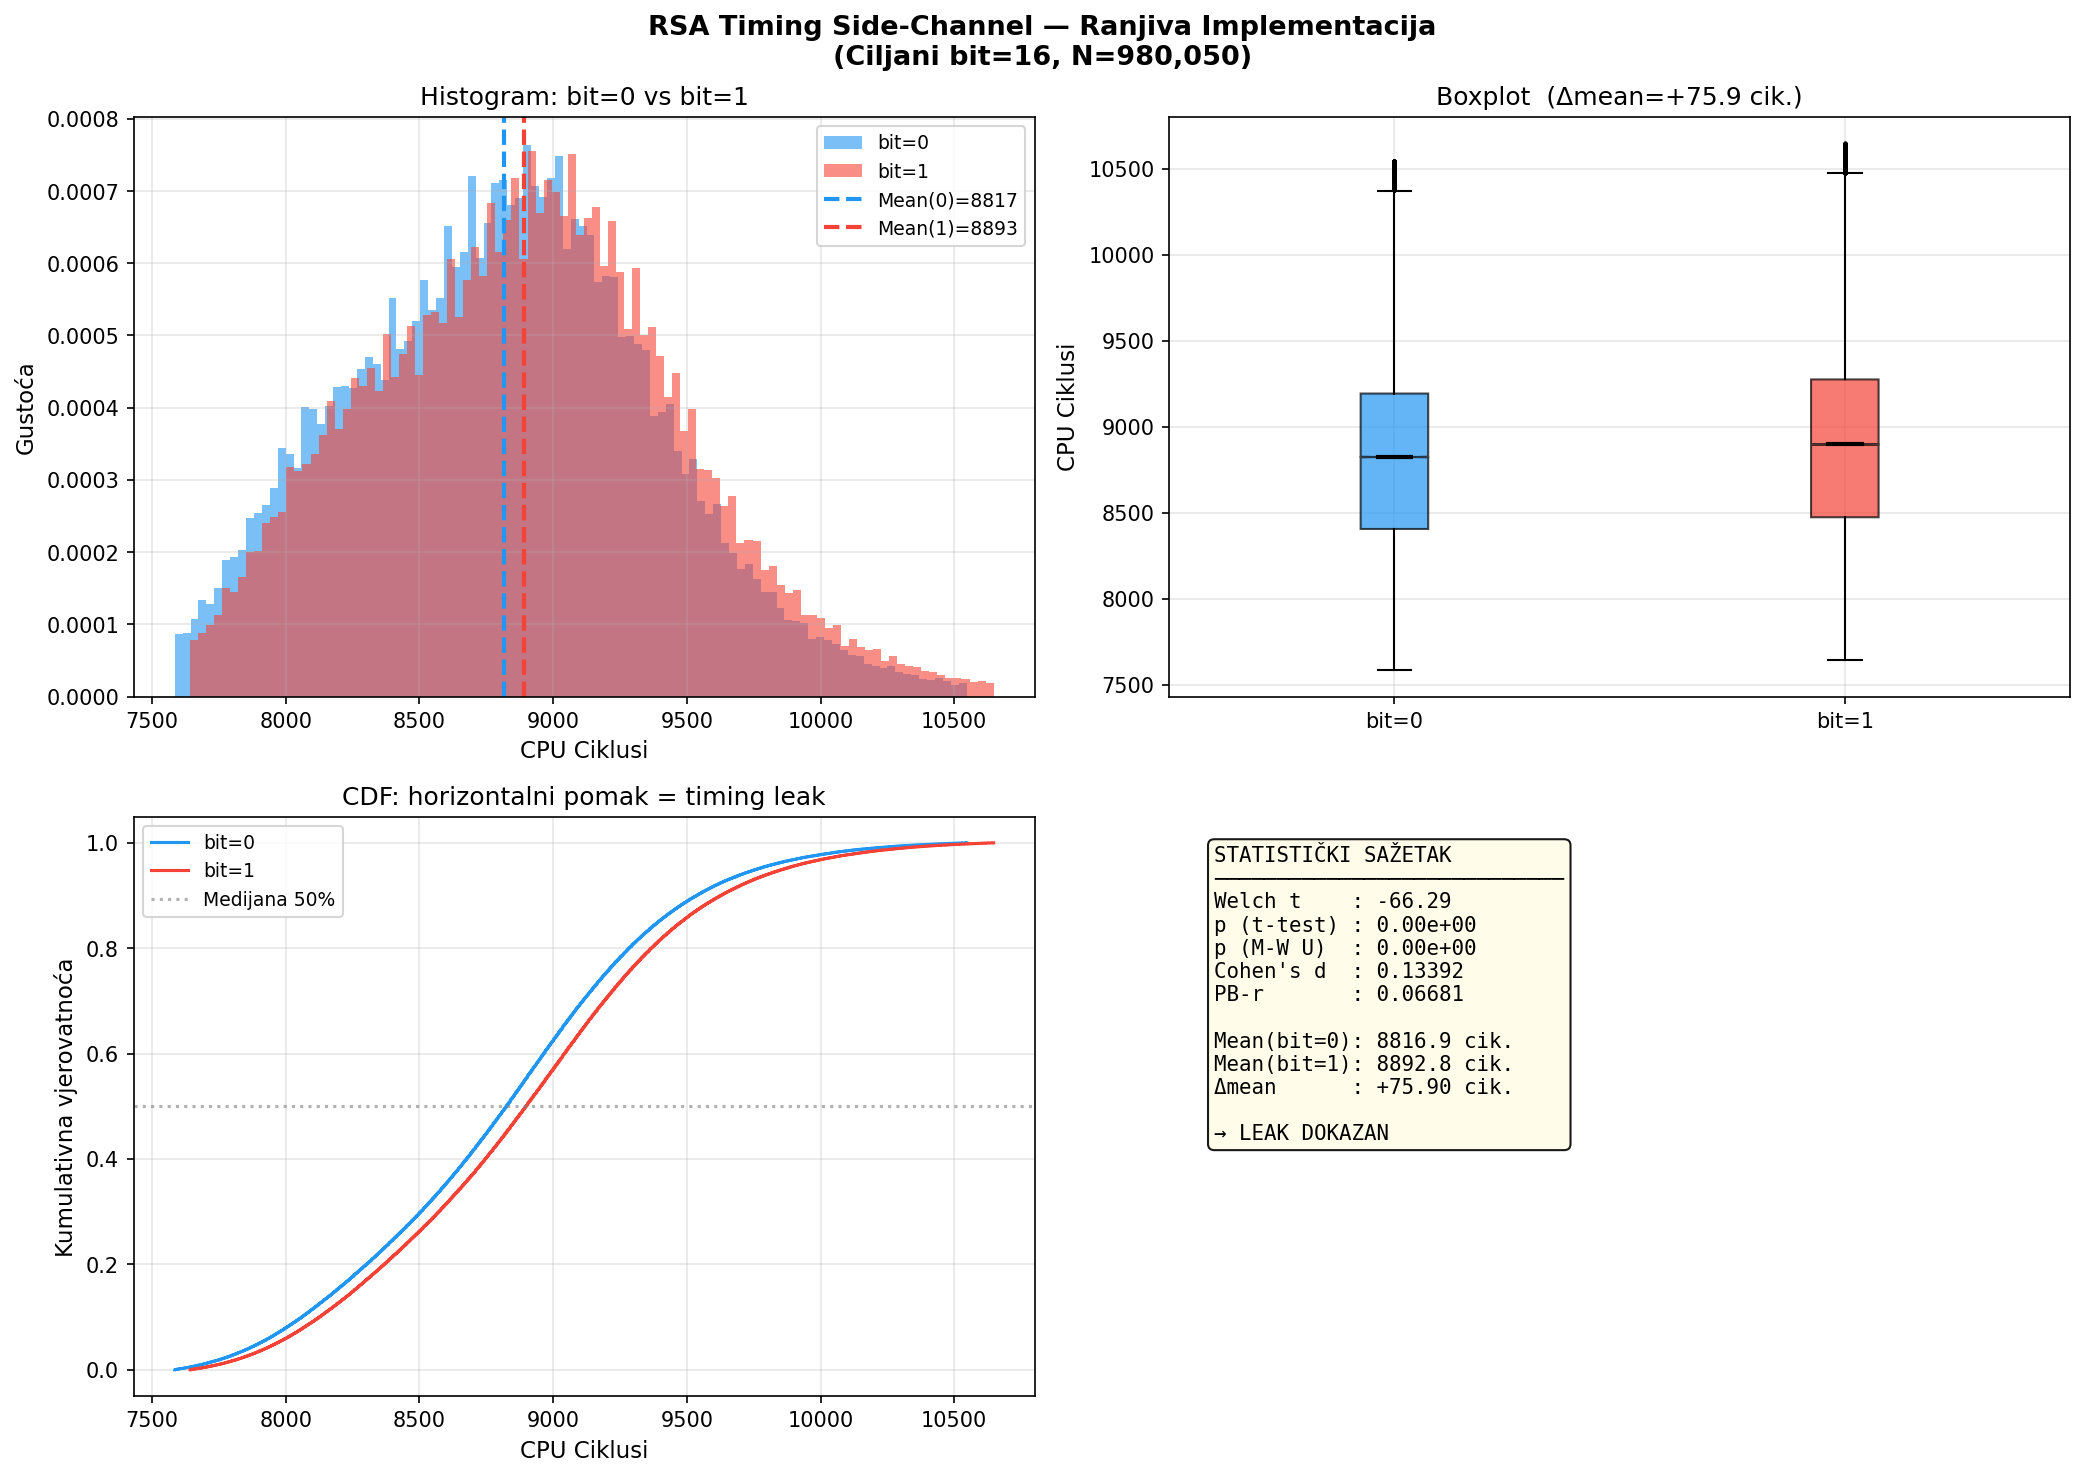
\includegraphics[width=\textwidth]{plot_vulnerable_analysis.png}
\caption{Distribucija trajanja ranjive implementacije: histogram, boxplot i CDF za grupe bit=0 i bit=1.}
\label{fig:vuln_analysis}
\end{figure}

Na slici \ref{fig:vuln_analysis} histogram prikazuje dvije distribucije koje se gotovo potpuno preklapaju, ali s vidljivim horizontalnim pomakom od oko 75 ciklusa. Preklapanje je očekivano s obzirom na mali Cohen-ov $d$: šum (varijansa od cache miss-ova, branch mispredictions i preempcija operativnog sistema) je znatno veći od signala. CDF (kumulativna funkcija distribucije) krivulje jasno ilustruju vremensko curenje: za isti postotak uzoraka, distribucija grupe bit=1 konzistentno zahtijeva veći broj ciklusa. Paralelnost CDF krivulja potvrđuje da je pomak uniforman preko cijele distribucije, a ne lokaliziran na određenom dijelu.

\begin{figure}[H]
\centering
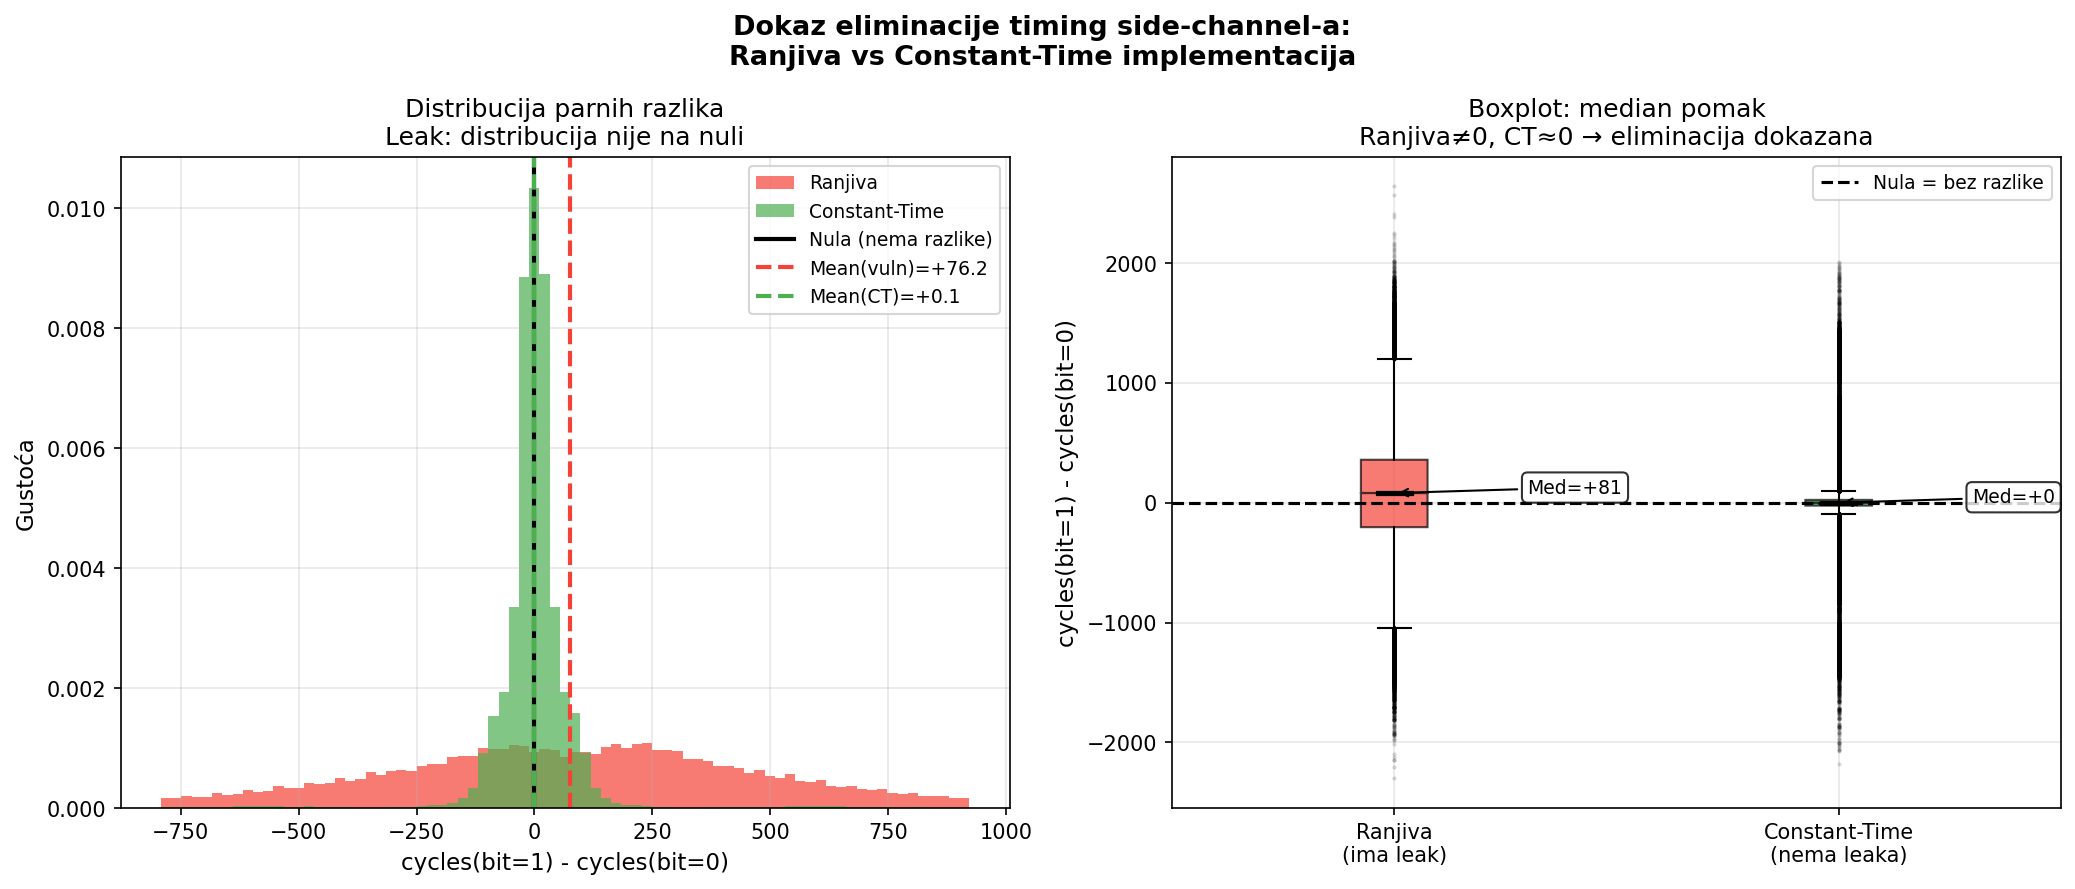
\includegraphics[width=\textwidth]{plot_comparison.png}
\caption{Distribucija parnih razlika trajanja za ranjivu (crvena) i konstantnu vremensku (zelena) implementaciju.}
\label{fig:comparison}
\end{figure}

Slika \ref{fig:comparison} direktno prikazuje distribuciju razlika unutar svakoga para. Za ranjivu implementaciju, centar distribucije je jasno pomaknut udesno od nule (centar na +76 ciklusa), dok za constant-time implementaciju distribucija leži precizno na nuli. Ovo je najintuitivniji vizualni dokaz da implementacija s konstantnim vremenom uspješno eliminiše curenje.

\subsection{Validacija eksperimenta}

Tabela \ref{tab:validation} sumira sedam unaprijed definisanih validacionih kriterija koji zajedno potvrđuju ispravnost eksperimentalnog postupka.

\begin{table}[H]
\centering
\caption{Validacija eksperimenta: svi kriteriji ispunjeni}
\label{tab:validation}
\begin{tabular}{lll}
\toprule
\textbf{Kriterij} & \textbf{Uslov} & \textbf{Rezultat} \\
\midrule
Vremensko curenje postoji & $p_{\text{MW}} < 10^{-10}$ & $< 10^{-50}$ \checkmark \\
T-test značajan & $p < 0{,}01$ & $< 10^{-50}$ \checkmark \\
Efekt mjerljiv & $|d| > 0{,}01$ & $d = 0{,}134$ \checkmark \\
Napad uspješan & tačnost $> 70\%$ & $100\%$ za $K = 2000$ \checkmark \\
CT eliminira leak & $p_{\text{MW}} > 0{,}05$ & $p = 0{,}327$ \checkmark \\
CT bez efekta & $|d| < 0{,}05$ & $d \approx 0{,}000$ \checkmark \\
CT napad neuspješan & tačnost $< 60\%$ & $\approx 50\%$ \checkmark \\
\bottomrule
\end{tabular}
\end{table}

Ispunjenje svih sedam kriterija potvrđuje da eksperimentalni postupak ispravno detektuje vremensko curenje kada postoji, i ispravno ne detektuje ništa kada ga nema. Ovo isključuje mogućnost da su rezultati posljedica metodološke greške.

% ---------------------------------------------------------------

\section{Eksperiment 2: Napad sa usrednjavanjem}
\label{sec:exp2}

\subsection{Metodologija}

Eksperiment 1 dokazuje da vremensko curenje postoji, ali postavlja se pitanje: može li napadač praktično iskoristiti signal od samo 76 ciklusa u šumu od 567 ciklusa za pogađanje vrijednosti tajnog bita? Eksperiment odgovara na ovo pitanje tako što demonstrira da usrednjavanje više mjerenja ignoriše šum i izvlači signal.

Za svaki nivo usrednjavanja K, napadač izvodi sljedeći postupak: (1) procjenjuje optimalni prag iz prve polovice podataka, (2) formira K nasumičnih mjerenja iz testnog skupa i računa njihovu sredinu, te (3) klasificira usrednjeni rezultat pravilom praga: ako je sredina iznad praga, proglašava bit=1, inače bit=0.

Teorijski minimalan K za postizanje 95\% tačnosti izvodi se iz odnosa signala i šuma. Za SNR $= d = 0{,}134$ i faktor pouzdanosti $r = 2$ (koji odgovara 95\% jednosmjernoj pouzdanosti, jednačina \ref{eq:kmin} daje $K_{\min} = (r/\text{SNR})^2 = (2/0{,}134)^2 \approx 223$. Intuicija iza ove formule je da standardna devijacija sredine od K mjerenja je $\sigma/\sqrt{K}$, pa sa dovoljno velikim K sredina postaje dovoljno precizna da signal od 76 ciklusa bude jasno odvojen od šuma.

\subsection{Rezultati}

\begin{table}[H]
\centering
\caption{Tačnost timing napada sa usrednjavajem u funkciji broja usrednjenih mjerenja K}
\label{tab:averaging}
\begin{tabular}{rrrr}
\toprule
\textbf{K} & \textbf{Tačnost (ranjiva)} & \textbf{95\% CI} & \textbf{Tačnost (CT)} \\
\midrule
1      & 53{,}4\% & [51{,}9\%, 54{,}9\%] & 50{,}2\% \\
10     & 57{,}8\% & [56{,}3\%, 59{,}3\%] & 50{,}0\% \\
100    & 74{,}6\% & [73{,}2\%, 75{,}9\%] & 50{,}9\% \\
500    & 92{,}4\% & [90{,}6\%, 93{,}9\%] & 50{,}9\% \\
1000   & 97{,}6\% & [95{,}8\%, 98{,}6\%] & 52{,}2\% \\
2000   & 100{,}0\% & [98{,}4\%, 100{,}0\%] & 43{,}9\% \\
5000   & 100{,}0\% & [96{,}2\%, 100{,}0\%] & 51{,}0\% \\
\bottomrule
\end{tabular}
\end{table}

\begin{figure}[H]
\centering
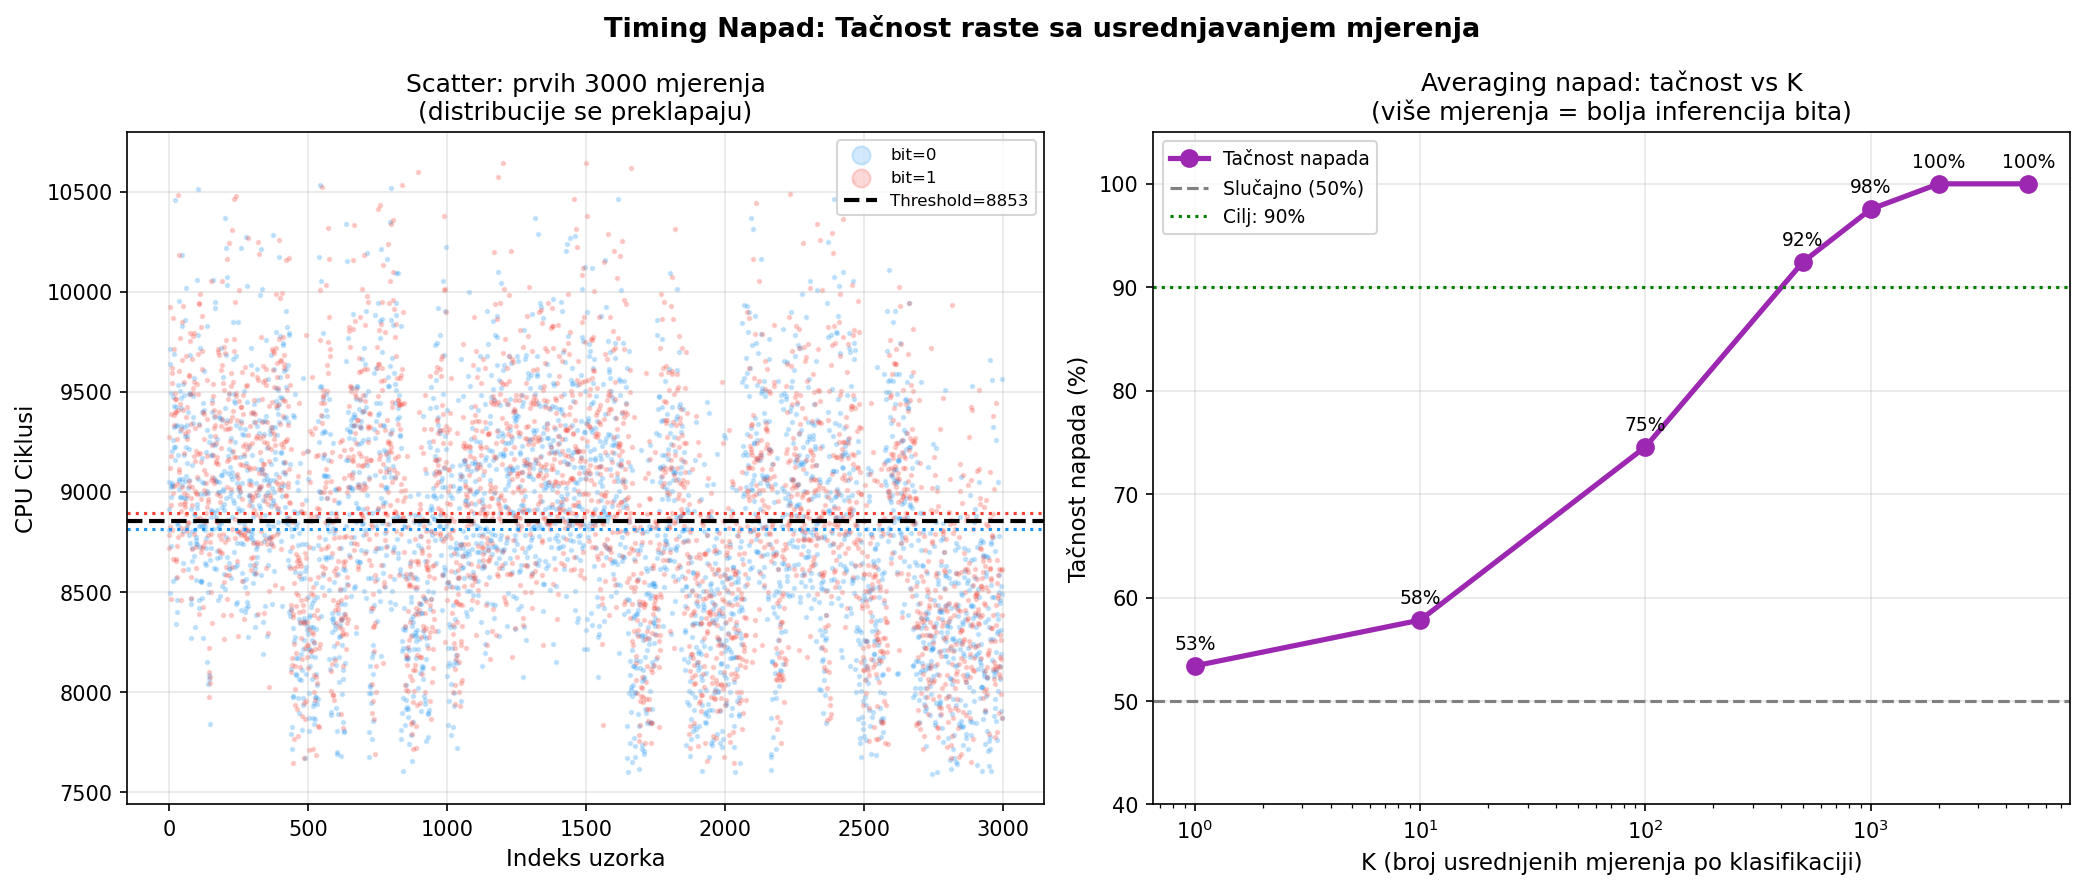
\includegraphics[width=\textwidth]{plot_inference_attack.png}
\caption{Dijagram raspršenja (\textit{scatter plot}) mjerenja (lijevo) i tačnost u funkciji K (desno).}
\label{fig:inference}
\end{figure}

Slika \ref{fig:inference} prikazuje rasipanje pojedinačnih mjerenja (lijevo) i rast tačnosti s povećanjem K (desno). Rezultati potvrđuju teorijsko predviđanje. Sa jednim mjerenjem ($K=1$), napadač pogađa tek 53{,}4\%, jedva iznad slučajnog pogađanja od 50\%, jer je signal zakopan u šumu. Sa $K = 100$, tačnost raste na 74{,}6\%, što je blizu teorijskog $K_{\min} = 223$ za 95\%. Sa $K = 500$ napadač postiže 92{,}4\%, a sa $K = 2000$ dostiže savršenih 100\%.

Fizičko objašnjenje: za $K = 2000$, standardna devijacija sredine iznosi $\sigma_{2000} = 567/\sqrt{2000} \approx 12{,}7$ ciklusa. Signal od 76 ciklusa je sada šest puta veći od šuma sredine, što čini pogrešnu klasifikaciju praktično nemogućom.

Za implementaciju s konstantnim vremenom tačnost napada ostaje u opsegu 44--52\% za sve vrijednosti K, što je konzistentno s odsustvom vremenskog curenja. Vrijednost od 43{,}9\% za $K = 2000$ je statističko odstupanje; 95\% interval povjerenja za slučajno pogađanje s 200--500 test blokova obuhvata ovaj raspon.

\subsection{Osjetljivost na veličinu uzorka}

Tabela \ref{tab:sensitivity} prikazuje kako se statistička značajnost i tačnost napada mijenjaju kada se koristi samo podskup ukupnih podataka. Ova analiza odgovara na pitanje: koliko mjerenja napadač minimalno treba prikupiti?
\begin{table}[H]
\centering
\caption{Osjetljivost na veličinu uzorka: p-vrijednost i tačnost napada}
\label{tab:sensitivity}
\begin{tabular}{rrrr}
\toprule
\textbf{N uzoraka} & \textbf{p-vrijednost} & \textbf{Značajno?} & \textbf{Tačnost ($K = 100$)} \\
\midrule
100       & 4{,}53e-02  & Da    & N/A \\
500       & 1{,}76e-02  & Da    & 90{,}0\% \\
1\,000    & 2{,}65e-07  & Da    & 90{,}0\% \\
2\,000    & 3{,}85e-07  & Da    & 85{,}0\% \\
5\,000    & 1{,}68e-12  & Da    & 75{,}0\% \\
10\,000   & 6{,}14e-17  & Da    & 70{,}5\% \\
50\,000   & 7{,}81e-112 & Da    & 73{,}6\% \\
100\,000  & 3{,}50e-198 & Da    & 76{,}9\% \\
\bottomrule
\end{tabular}
\end{table}

Za $N = 100$, usrednjavanje sa $K = 100$ nije moguće jer ukupan broj uzoraka nije dovoljan za formiranje nezavisnih blokova, pa je tačnost označena kao N/A. Najmanji N za postizanje statističke značajnosti ($p < 0{,}05$) iznosi $N = 100$ ($p = 4{,}53 \times 10^{-2}$). Čak i sa samo 100 uzoraka timing leak je na granici statističke vidljivosti, uprkos tome što power analiza za 80\% snagu predviđa $N_{\min} = 438$. Ovo sugeriše da je stvarna veličina efekta u ovom poduzorku bila nešto veća od ukupnog prosjeka.

Naizgled paradoksalan pad tačnosti napada za veće $N$ (npr. 90\% za $N=500$ naspram 70{,}5\% za $N=10\,000$ uz $K=100$) objašnjava se nestabilnošću procjene pri malom broju test blokova. Za $N=500$ i $K=100$ postoji samo 5 nezavisnih blokova (svaki od 100 mjerenja), pa jedan ili dva sretna bloka značajno utječu na procijenjenu tačnost. Za veće $N$, broj blokova raste i procjena konvergira ka stvarnoj tačnosti od približno 75\% za $K=100$, što odgovara teorijskom predviđanju za SNR $= 0{,}134$ i $K$ daleko ispod $K_{\min} = 223$.

\begin{figure}[H]
\centering
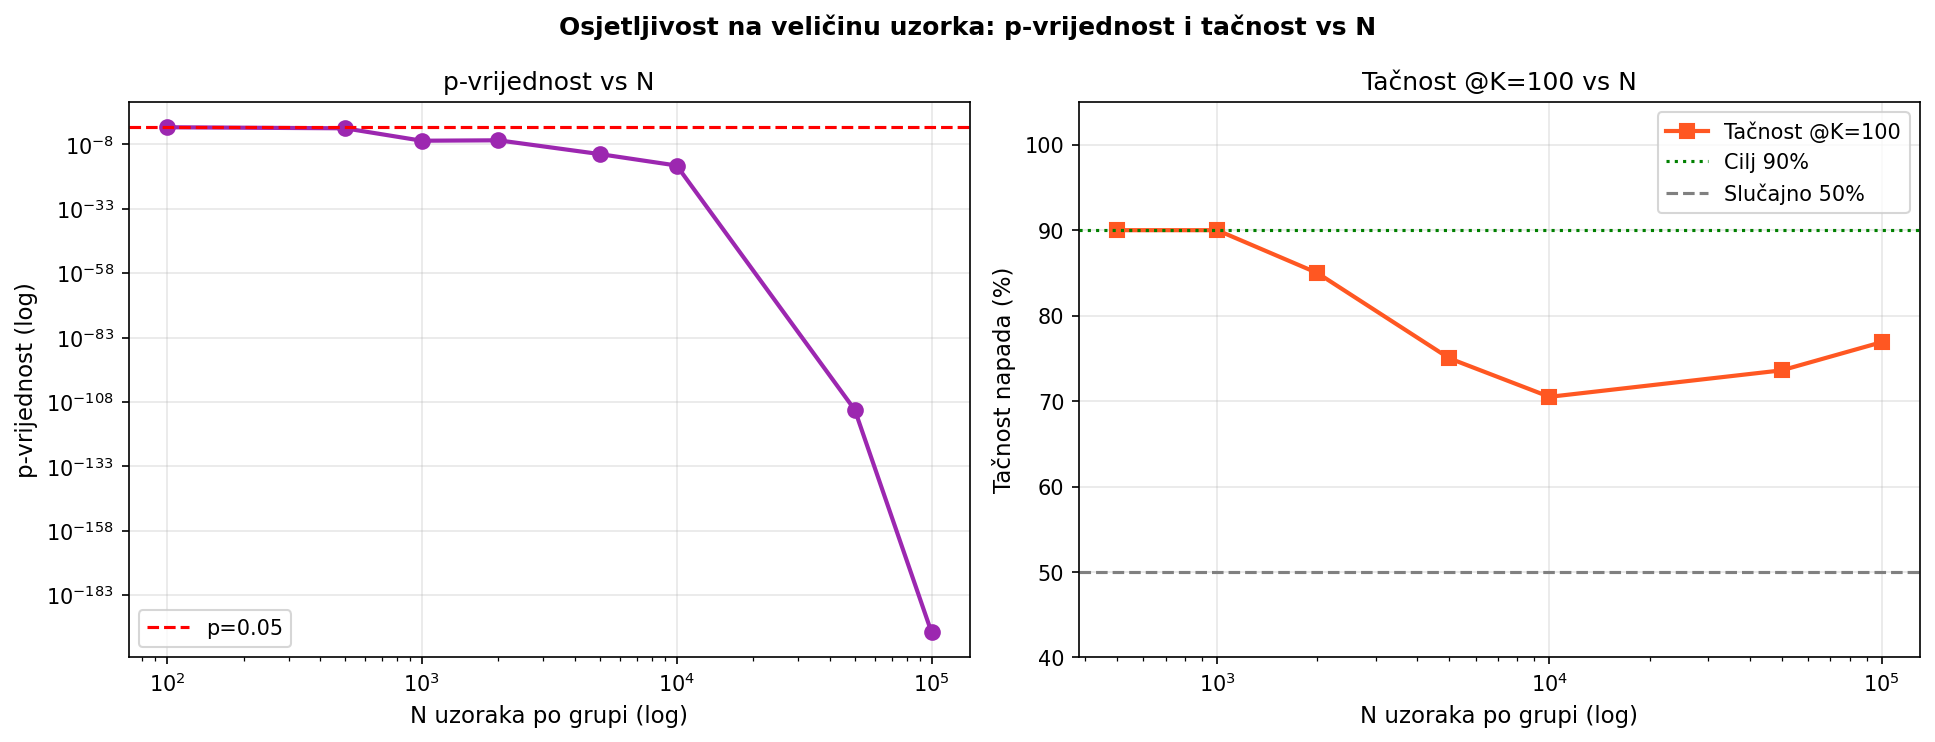
\includegraphics[width=\textwidth]{plot_sample_sensitivity.png}
\caption{Osjetljivost napada na veličinu uzorka: tačnost u funkciji $N$ za $K = 100$.}
\label{fig:sample_sensitivity}
\end{figure}

% ---------------------------------------------------------------

\section{Eksperiment 3: Slijepa rekonstrukcija 64-bitnog privatnog ključa}
\label{sec:exp3}

\subsection{Metodologija}

Eksperimenti 1 i 2 pokazuju da napadač može pouzdano odrediti vrijednost jednog bita. Eksperiment 3 primjenjuje isti princip na svih 64 bita privatnog ključa i rekonstruiše cijeli ključ, uz jedno ključno obilježje: napadački kod nikada ne vidi tajni ključ.

Tajni ključ generisan je nasumično iz \texttt{/dev/urandom} i pohranjen unutar zasebnog modula kome napadač nema direktan pristup (sekcija~\ref{sec:key_recon}). Za svaki bit napadač pita taj modul koliko dugo traje eksponencijacija s originalnim ključem i koliko bi trajala da je samo taj jedan bit obrnut. Iz razlike tih trajanja zaključuje koja je bila izvorna vrijednost bita. Ovaj postupak se ponavlja za sva 64 bita, sa $K = 5000$ mjerenja po bitu radi pouzdanosti. Tek na samom kraju, radi provjere tačnosti, modul otkriva tajni ključ.

\subsection{Rezultati}

\begin{table}[H]
\centering
\caption{Rezultati slijepe rekonstrukcije 64-bitnog ključa}
\label{tab:key_recon}
\begin{tabular}{ll}
\toprule
\textbf{Metrika} & \textbf{Vrijednost} \\
\midrule
Tajni ključ (nasumičan, \texttt{/dev/urandom}) & \texttt{0xAB568018B673C14C} \\
Rekonstruisani ključ                           & \texttt{0xAB568018B673C14C} \\
XOR razlika                                    & \texttt{0x0000000000000000} \\
Tačni biti                                     & 64 / 64 (100{,}0\%) \\
K po bitu                                      & 5\,000 \\
Mean $|\Delta|$                                & 73{,}1 ciklusa \\
Mean $\Delta$ (bit=1 pozicije)                 & $+$54{,}6 ciklusa \\
Mean $\Delta$ (bit=0 pozicije)                 & $-$87{,}4 ciklusa \\
\bottomrule
\end{tabular}
\end{table}

\begin{figure}[H]
\centering
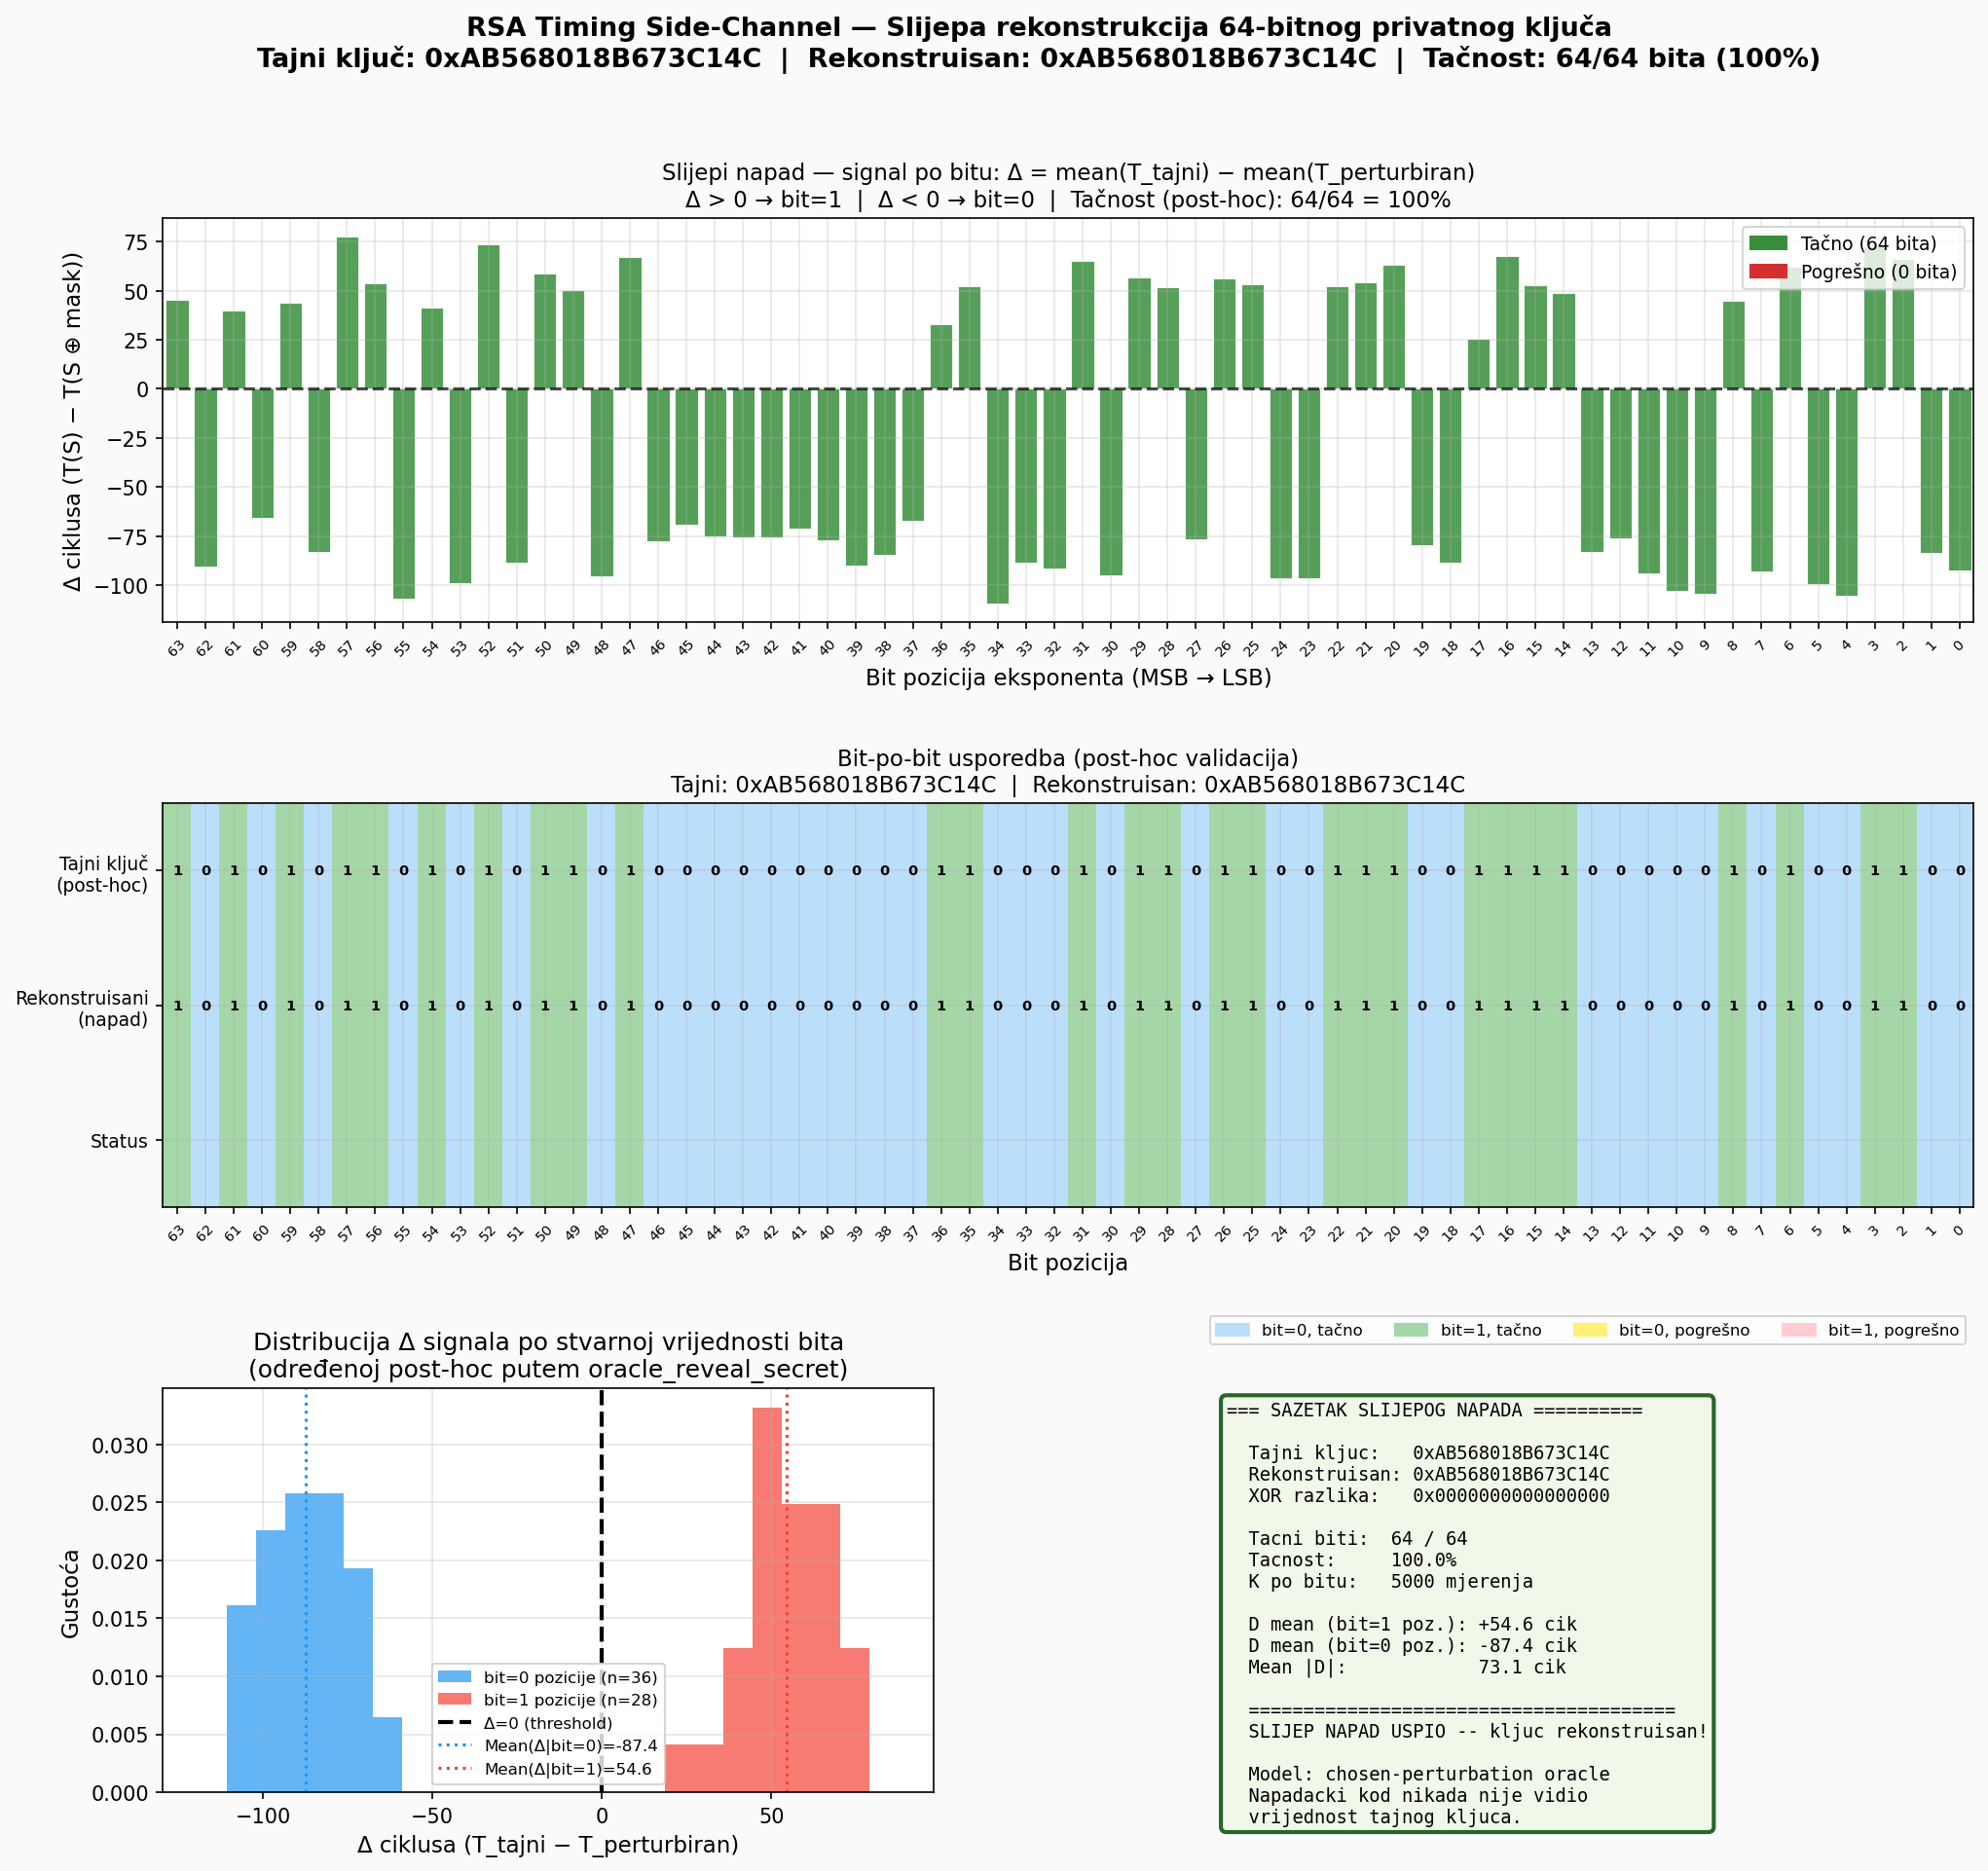
\includegraphics[width=\textwidth]{plot_key_reconstruction_blind.png}
\caption{Gornji panel: timing razlika $\Delta$ za svaki od 64 bita (pozitivna vrijednost = bit=1, negativna = bit=0). Srednji panel: toplotna mapa rekonstruisanog i stvarnog ključa. Donji panel: distribucija svih $\Delta$ vrijednosti}
\label{fig:key_recon}
\end{figure}

Kao što se vidi na slici \ref{fig:key_recon}, svih 64 bita nasumičnog tajnog ključa su tačno rekonstruisani. Timing razlika $\Delta$ je konzistentna i jasno odvojena po predznaku na svim pozicijama: pozicije gdje je tajni bit 1 daju pozitivan $\Delta$ (prosjek $+54{,}6$ ciklusa), a pozicije gdje je bit 0 daju negativan $\Delta$ (prosjek $-87{,}4$ ciklusa). Predznak $\Delta$ direktno otkriva vrijednost bita jer obrtanje bita iz 1 u 0 uklanja jedno množenje i skraćuje trajanje, dok obrtanje iz 0 u 1 dodaje množenje i produžava ga.

Veličina signala varira od pozicije do pozicije: najslabija razlika bila je 25{,}3 ciklusa (bit 17), a najjača 109{,}2 ciklusa (bit 34). Ova varijacija je normalna i odgovara rezultatima Eksperimenta 4. Ni za jedan bit nisu bila potrebna ponovna mjerenja: najmanji $|t|$-statistik iznosio je 8{,}3, daleko iznad praga od 2{,}5 koji bi aktivirao drugi prolaz.

Rekonstrukcija je potpuno zasnovana na timing mjerenjima i napadački kod u nijednom trenutku nije pristupio vrijednosti tajnog ključa. Ovo odgovara realnom napadu: server drži privatni ključ, a napadač ga može jedino posredno "posmatrati" kroz razlike u trajanju odgovora.

% ---------------------------------------------------------------

\section{Eksperiment 4: Analiza pozicije bita}

\subsection{Motivacija i metodologija}

Eksperimenti 1 i 2 ciljaju fiksiranu poziciju bita (bit 16), a Eksperiment 3 primjenjuje napad na svih 64 bita. Prirodno pitanje je: da li je vremensko curenje sistemska osobina koja važi za svaku poziciju, ili postoje pozicije gdje je signal slabiji? Odgovor na ovo pitanje je ključan jer napad rekonstrukcije ključa pretpostavlja da svaki bit nezavisno daje mjerljiv signal.

Eksperiment testira svaku od 64 pozicija bita nezavisno, sa 10\,000 uzoraka po poziciji, i za svaku izračunava Welch-ov t-test i Cohen-ov $d$.

\subsection{Rezultati}

\begin{table}[H]
\centering
\caption{Multi-bit sweep: ukupni rezultati}
\label{tab:sweep_summary}
\begin{tabular}{ll}
\toprule
\textbf{Metrika} & \textbf{Vrijednost} \\
\midrule
Statistički značajnih pozicija & 64 / 64 (100\%) \\
Mean $\Delta$ po svim bitovima & +75{,}67 ciklusa \\
Std $\Delta$ & 7{,}07 ciklusa \\
One-sample t-test ($H_0$: mean $\Delta = 0$) & $t = 84{,}993$,\ $p = 1{,}027 \times 10^{-66}$ \\
\bottomrule
\end{tabular}
\end{table}

\begin{figure}[H]
\centering
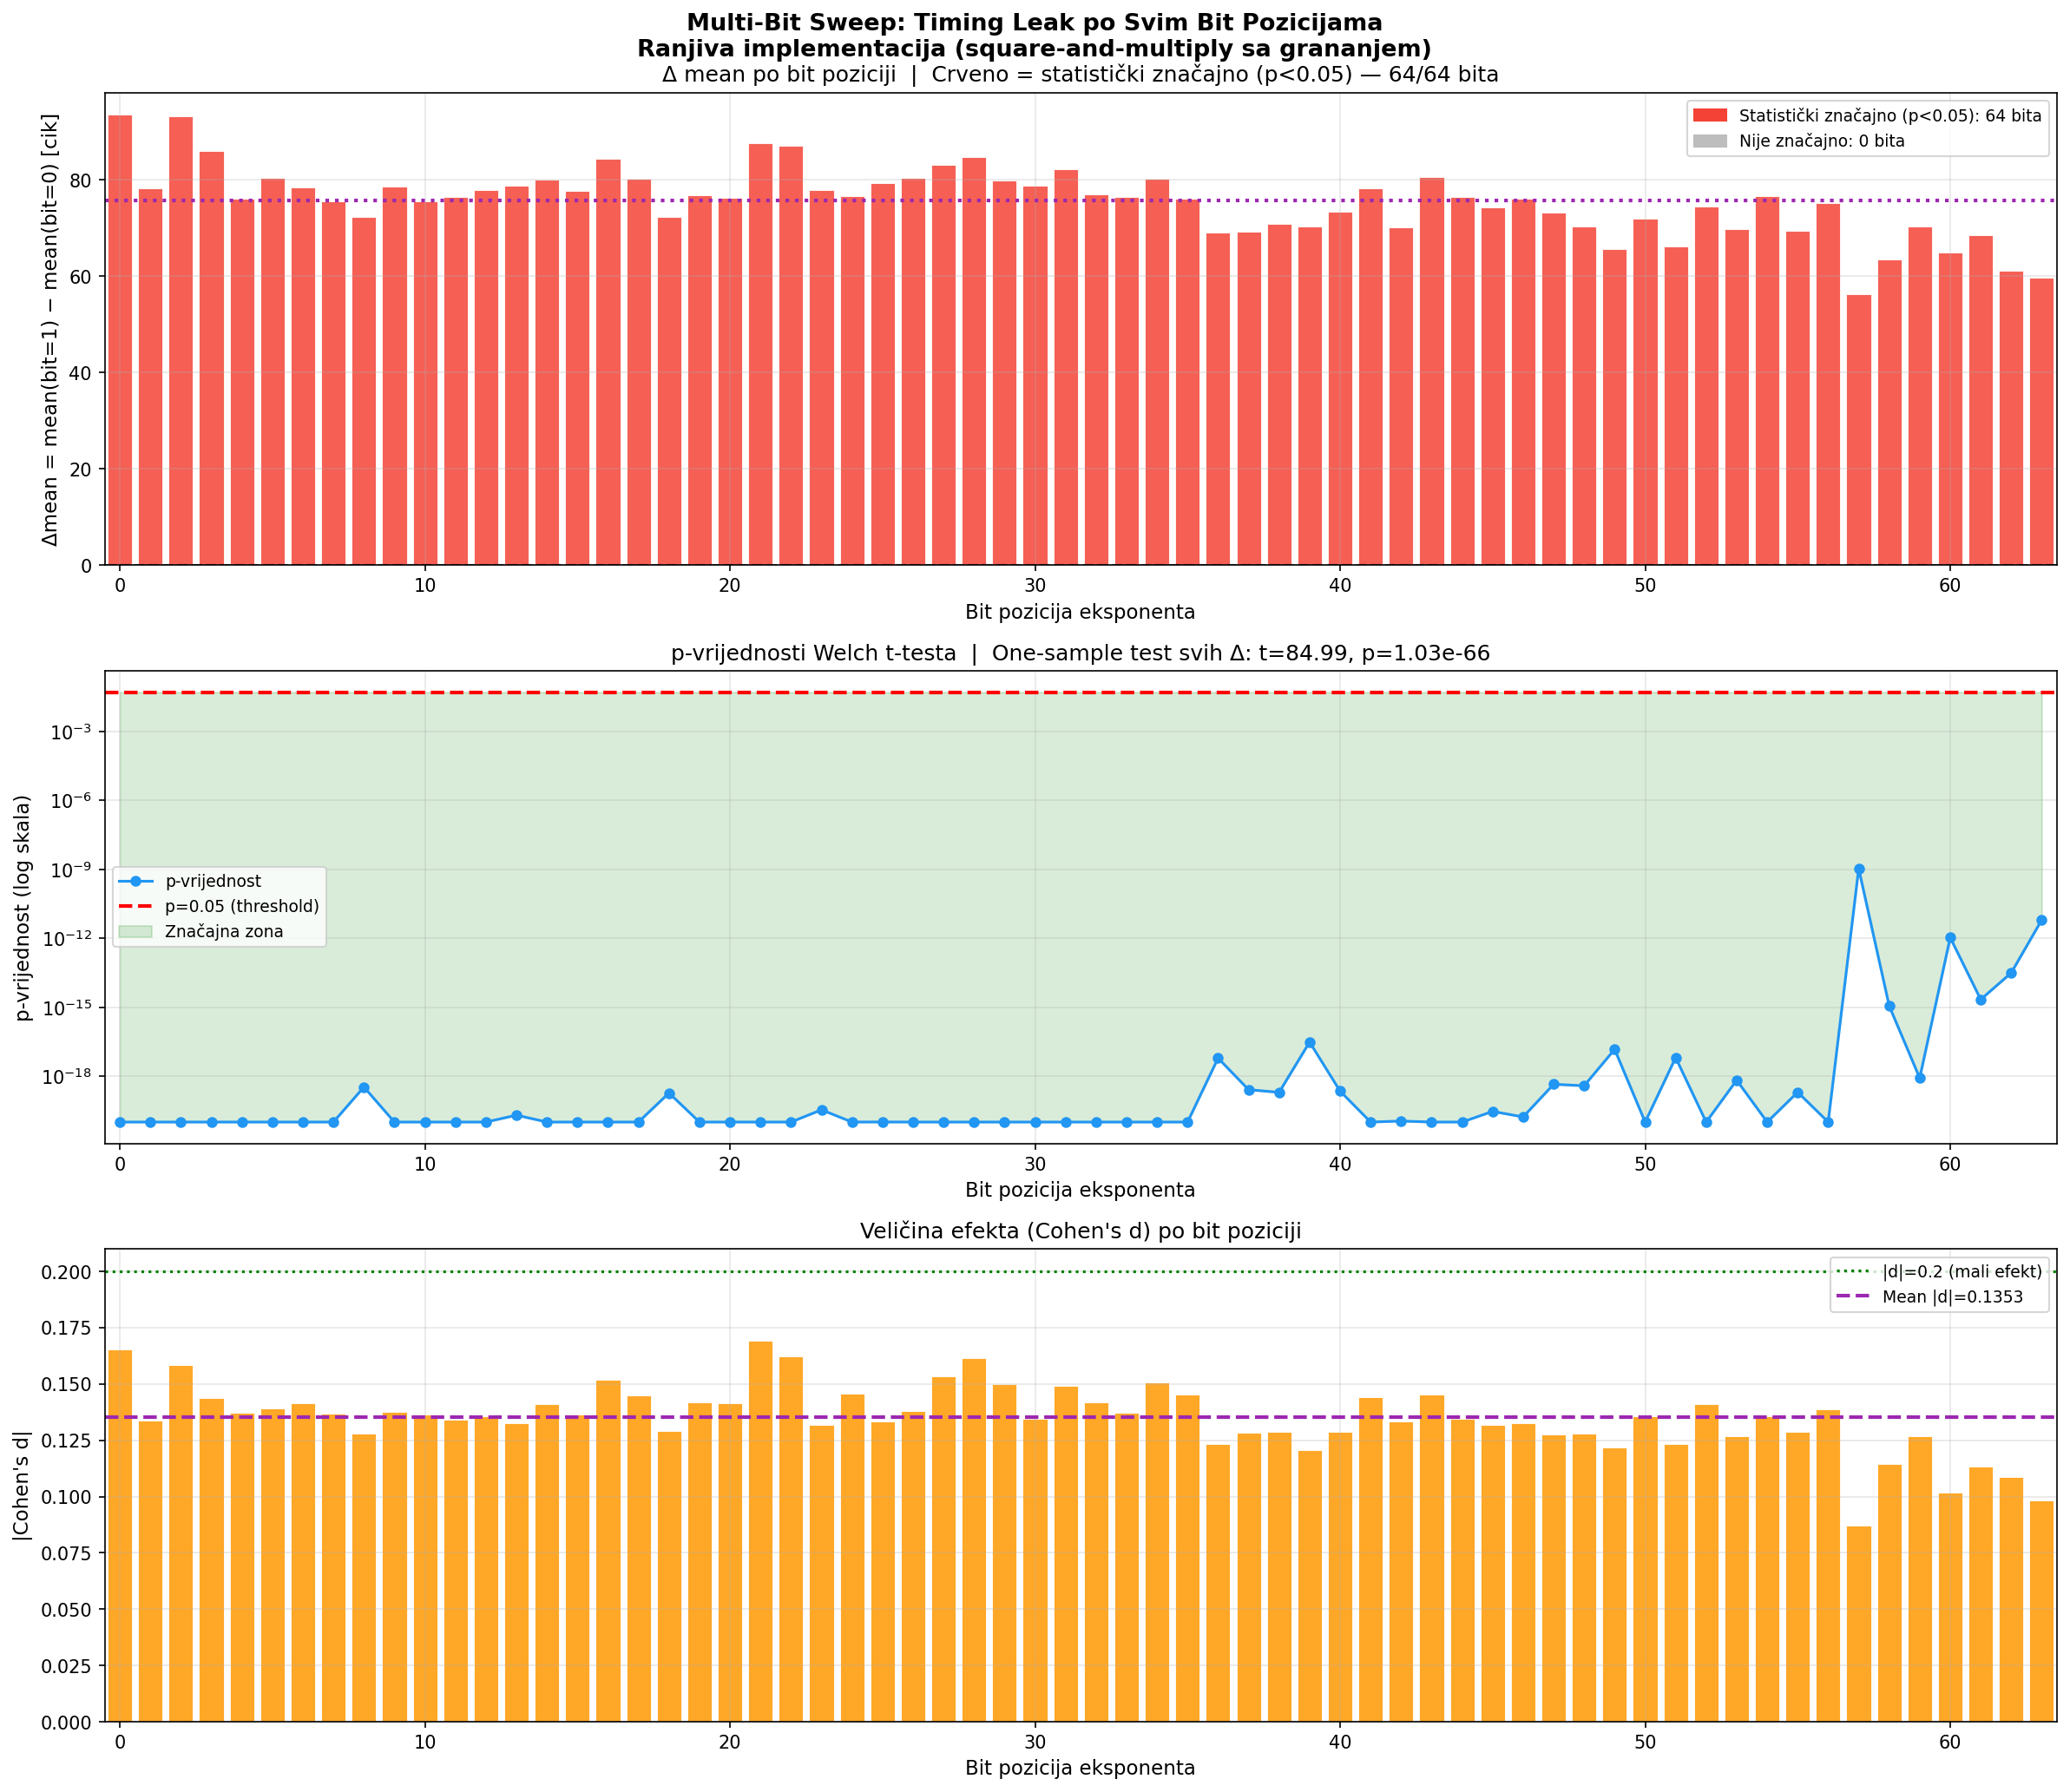
\includegraphics[width=\textwidth]{plot_multi_bit_sweep.png}
\caption{Timing razlika $\Delta$ po poziciji bita eksponenta sa 95\% intervalima povjerenja.}
\label{fig:sweep}
\end{figure}

Svih 64 pozicija bita pokazuju statistički značajnu vremensku razliku ($p < 10^{-9}$ za svaku poziciju pojedinačno). Prosječna razlika $\Delta$ kreće se od $+56{,}22$ ciklusa (bit 57) do $+93{,}49$ ciklusa (bit 0), sa ukupnom standardnom devijacijom od 7{,}07 ciklusa između pozicija.
\\

Varijacija $\Delta$ po poziciji (od 56 do 93 ciklusa) nije sistematski trend nego kontekstualni šum: svaka iteracija petlje zatekne različito stanje branch prediktora i cache memorije ovisno o tome koji su se bitovi izvršili ranije, što uvodi slučajnu varijabilnost u izmjerenu razliku. Minimalna vrijednost na bitu 57 i maksimalna na bitu 0 su primjer te slučajnosti i ne postoji krivulja koja pada ili raste s pozicijom. Za realni 2048-bitni ključ slika bi izgledala isto: oko 2048 tačaka grupisanih oko iste srednje vrijednosti (~75 ciklusa) s jednakom slučajnom rasutošću. Standardna devijacija od samo 7{,}07 ciklusa (naspram srednje vrijednosti od 75{,}67) potvrđuje visoku konzistentnost signala bez obzira na poziciju.
\\

One-sample t-test svih 64 delta vrijednosti daje $t = 84{,}993$ ($p = 1{,}027 \times 10^{-66}$), čime se definitivno odbacuje hipoteza da je prosječna razlika jednaka nuli. Ovaj rezultat potvrđuje da vremensko curenje nije nastalo zbog jedne bit pozicije, već je osobina ranjive square-and-multiply implementacije: svaki bit eksponenta nezavisno doprinosi mjerljivoj vremenskoj razlici.

% ---------------------------------------------------------------

\section{Eksperiment 5: Utjecaj kompajlerskih optimizacija}
\label{sec:compiler_exp}

\subsection{Motivacija}

U sekciji \ref{sec:vuln_impl} navedeno je da ranjiva implementacija koristi \texttt{optimize("O0")} atribut koji isključuje optimizacije. Postavlja se praktično pitanje: može li kompajler s višim nivoom optimizacije automatski eliminisati timing leak, na primjer transformacijom uslovnog grananja (\texttt{if}) u instrukciju uslovnog pomaka (\texttt{CMOV}) koja se izvršava u konstantnom vremenu? Ako bi to bio slučaj, programeri bi se mogli osloniti na kompajler umjesto na eksplicitne kontramjere.

Ovaj eksperiment testira pet varijanti iste ranjive implementacije kompajlirane s različitim optimizacijskim nivoima i provjerava generisani asemblerski kod.

\subsection{Rezultati}

\begin{table}[H]
\centering
\caption{Timing leak po nivoima kompajlerske optimizacije}
\label{tab:compiler}
\begin{tabular}{llrrrrl}
\toprule
\textbf{Varijanta} & \textbf{Opt.} & \textbf{Atribut} & \textbf{$\Delta$ mean} & \textbf{p-vrijednost} & \textbf{Cohen-ov $d$} & \textbf{Assembly} \\
\midrule
O0       & \texttt{-O0} & Ne  & +77{,}29 & $< 10^{-50}$ & 0{,}136 & branch \\
O1       & \texttt{-O1} & Ne  & +72{,}01 & $< 10^{-50}$ & 0{,}267 & branch \\
O2       & \texttt{-O2} & Ne  & +71{,}73 & $< 10^{-50}$ & 0{,}267 & branch \\
O3       & \texttt{-O3} & Ne  & +71{,}83 & $< 10^{-50}$ & 0{,}267 & branch \\
O2+attr  & \texttt{-O2} & Da  & +77{,}62 & $< 10^{-50}$ & 0{,}120 & branch \\
\bottomrule
\end{tabular}
\end{table}

\begin{figure}[H]
\centering
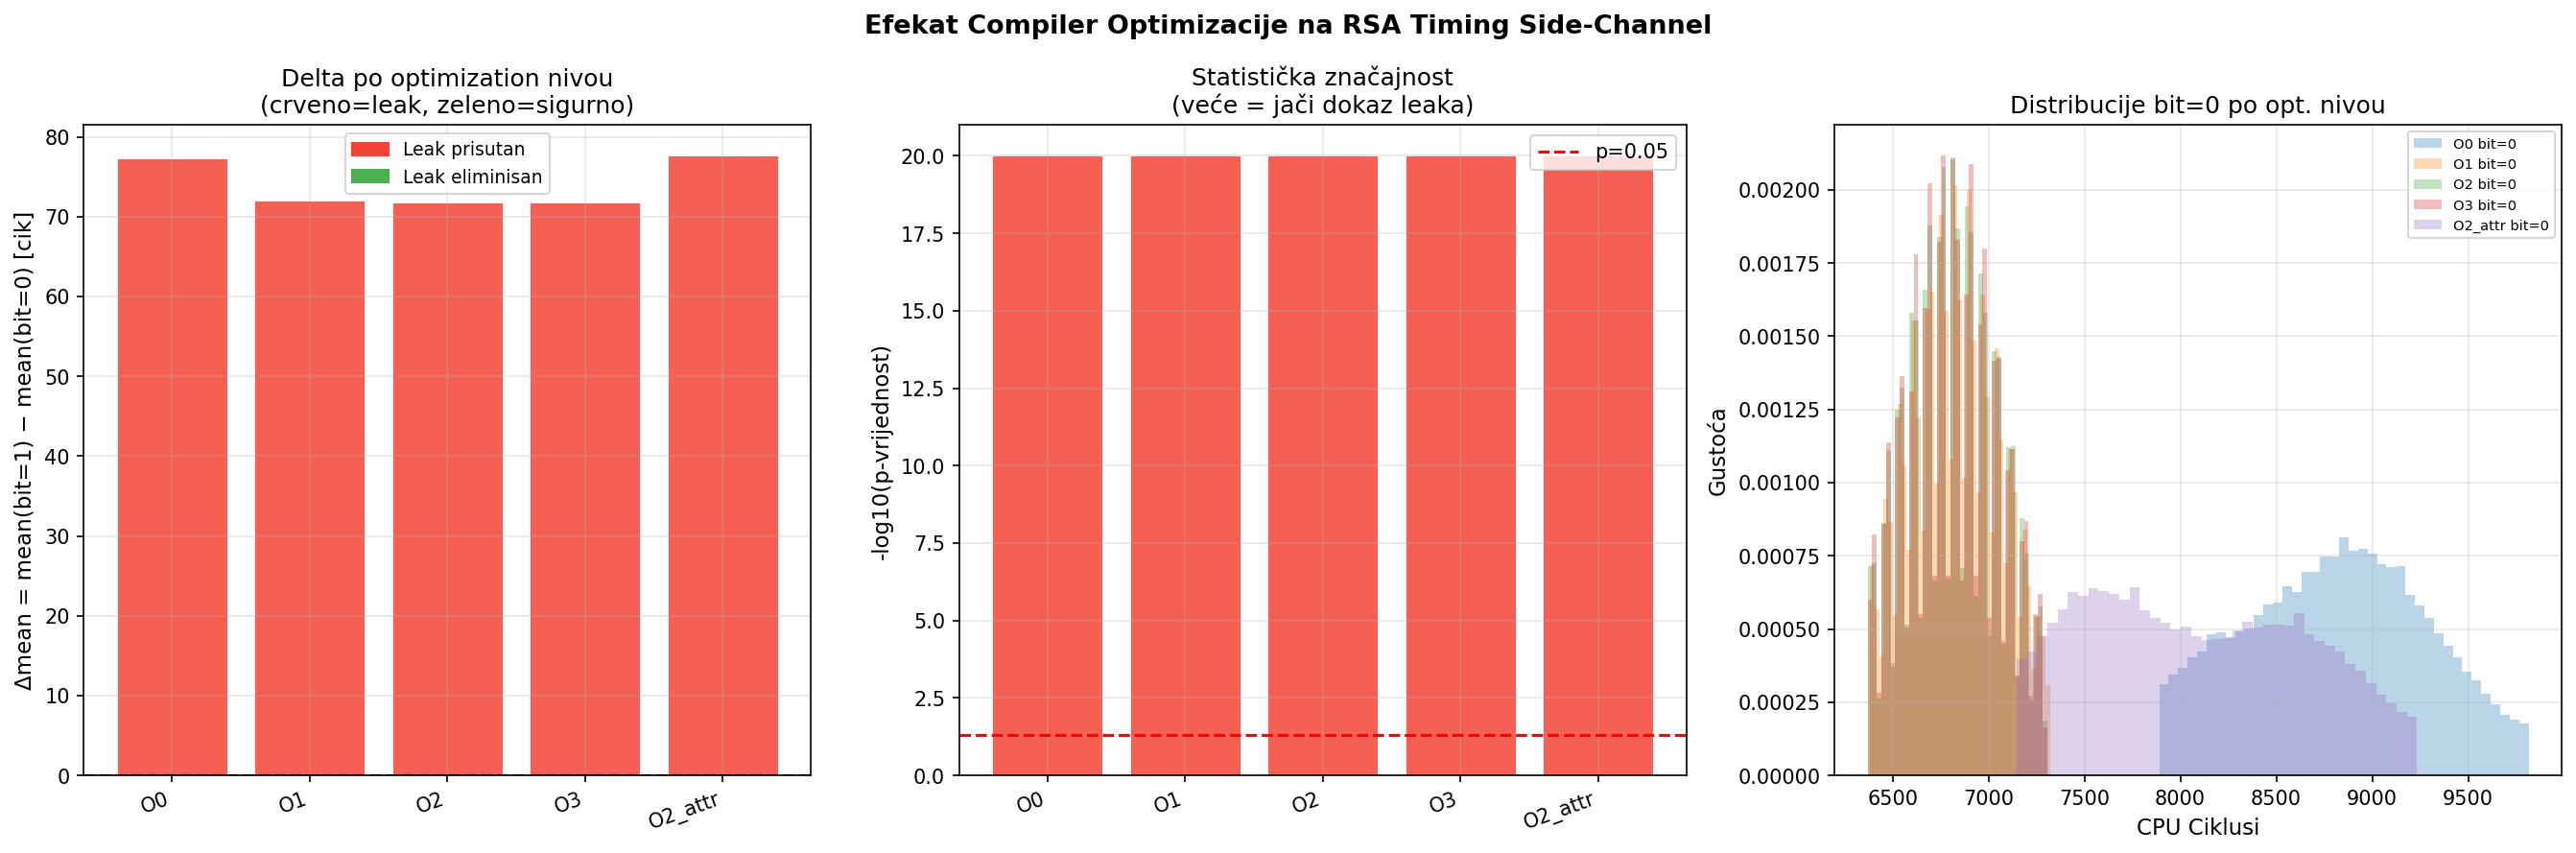
\includegraphics[width=\textwidth]{plot_compiler_effects.png}
\caption{Utjecaj kompajlerskih optimizacija: prosječna timing razlika $\Delta$ (u CPU ciklusima) i Cohen-ov $d$ za pet varijanti ranjive implementacije.}
\label{fig:compiler}
\end{figure}

Nijedan nivo optimizacije ne eliminiše vremensko curenje. Pregled asemblerskog koda za sve varijante (vidjeti Prilog \ref{app:asm_output}) potvrđuje da GCC ne transformiše grananje u \texttt{CMOV} instrukciju ni za jedan nivo optimizacije, a razlog je tehničke prirode: tijelo uslovnog bloka sadrži poziv funkcije (\texttt{mulmod}), a \texttt{CMOV} može zamijeniti samo jednostavne dodjele vrijednosti, ne pozive funkcija. Pri \texttt{-O0} i \texttt{O2+attr} kompajler generiše \texttt{je} (obrazac \texttt{shrx}/\texttt{and}/\texttt{test}/\texttt{je}), a pri \texttt{-O1}--\texttt{-O3} generiše \texttt{jae} (obrazac \texttt{bt}/\texttt{jae}); u oba slučaja radi se o uslovnom skoku koji mijenja putanju izvršavanja ovisno o vrijednosti tajnog bita.

Zanimljiv nalaz je da optimizacije \texttt{-O1} do \texttt{-O3} zapravo pojačavaju vremensku razliku Cohen-ov $d$ raste sa 0{,}136 (O0) na 0{,}267 (O1--O3), što je gotovo dvostruko povećanje. Fizičko objašnjenje: optimizirani kod drži varijable u registrima umjesto na steku i generiše kompaktniji pristup memoriji, što smanjuje ukupnu varijansu ($\sigma$). Budući da je signal ($\Delta \approx 72$ ciklusa) gotovo isti, manji šum daje veći odnos signala i šuma (SNR).

Varijanta ``O2+attr'' koristi \texttt{-O2} nivo za cijeli program, ali ciljanu funkciju označava atributom \texttt{optimize("O0")}. Ova varijanta ima nešto veći $\Delta$ (+77{,}62 naspram +71{,}73) ali manji Cohen-ov $d$ (0{,}120) jer neoptimizirana funkcija ima veću varijansu.

Ovaj eksperiment demonstrira da se programeri ne mogu osloniti na kompajlerske optimizacije kao sigurnosnu mjeru. Jedino eksplicitne vremenski konstantne implementacije, poput one opisane u sekciji \ref{sec:ct_impl}, garantuju odsustvo vremenskog curenja neovisno o kompajleru i nivou optimizacije.

% ---------------------------------------------------------------

\section{Eksperiment 6: Evaluacija RSA blindinga}

\subsection{Motivacija}

RSA blinding je kontramjera koju je OpenSSL implementirao nakon Brumley-Boneh napada \cite{brumley2003}. Principi standardnog RSA blindinga opisani su u sekciji \ref{sec:blinding_theory}. U ovom eksperimentu korištena je pojednostavljena varijanta blindinga:
\begin{align}
\text{blinded\_base} &= M \cdot r \bmod n \\
s' &= \text{blinded\_base}^d \bmod n
\end{align}

Unblinding u ovoj varijanti nije matematički egzaktan jer $(M \cdot r)^d \neq M^d \cdot r$, ali za analizu timing signala ispravnost krajnjeg rezultata nije relevantna. Ovaj pristup je validan jer mjerimo isključivo trajanje operacije eksponencijacije, ne njen izlaz, a nasumičan odabir baze vjerno replicira efekat blindinga na interne međuvrijednosti tokom eksponencijacije. Konkretno, promjenom baze mijenjaju se svi međurezultati tokom eksponencijacije, što je suštinski jednak efekt onome što standardni blinding postiže na vremensku distribuciju iako konačni rezultat nije matematički egzaktan dekript.

Eksperiment poredi blinded i unblinded varijantu sa oko 196\,000 uzoraka po varijanti.

\subsection{Rezultati}

\begin{table}[H]
\centering
\caption{Evaluacija RSA blindinga kao kontramjere}
\label{tab:blinding}
\begin{tabular}{lrrrrrl}
\toprule
\textbf{Varijanta} & \textbf{N} & \textbf{$\Delta$} & \textbf{t-stat} & \textbf{p-vrijednost} & \textbf{Cohen-ov $d$} & \textbf{Štiti?} \\
\midrule
Blinded     & 195\,999 & +65{,}30 & $-30{,}78$ & $9{,}3 \times 10^{-208}$ & 0{,}098 & Ne \\
Unblinded   & 196\,035 & +75{,}03 & $-39{,}15$ & $< 10^{-50}$              & 0{,}125 & Ne \\
\bottomrule
\end{tabular}
\end{table}

\begin{figure}[H]
\centering
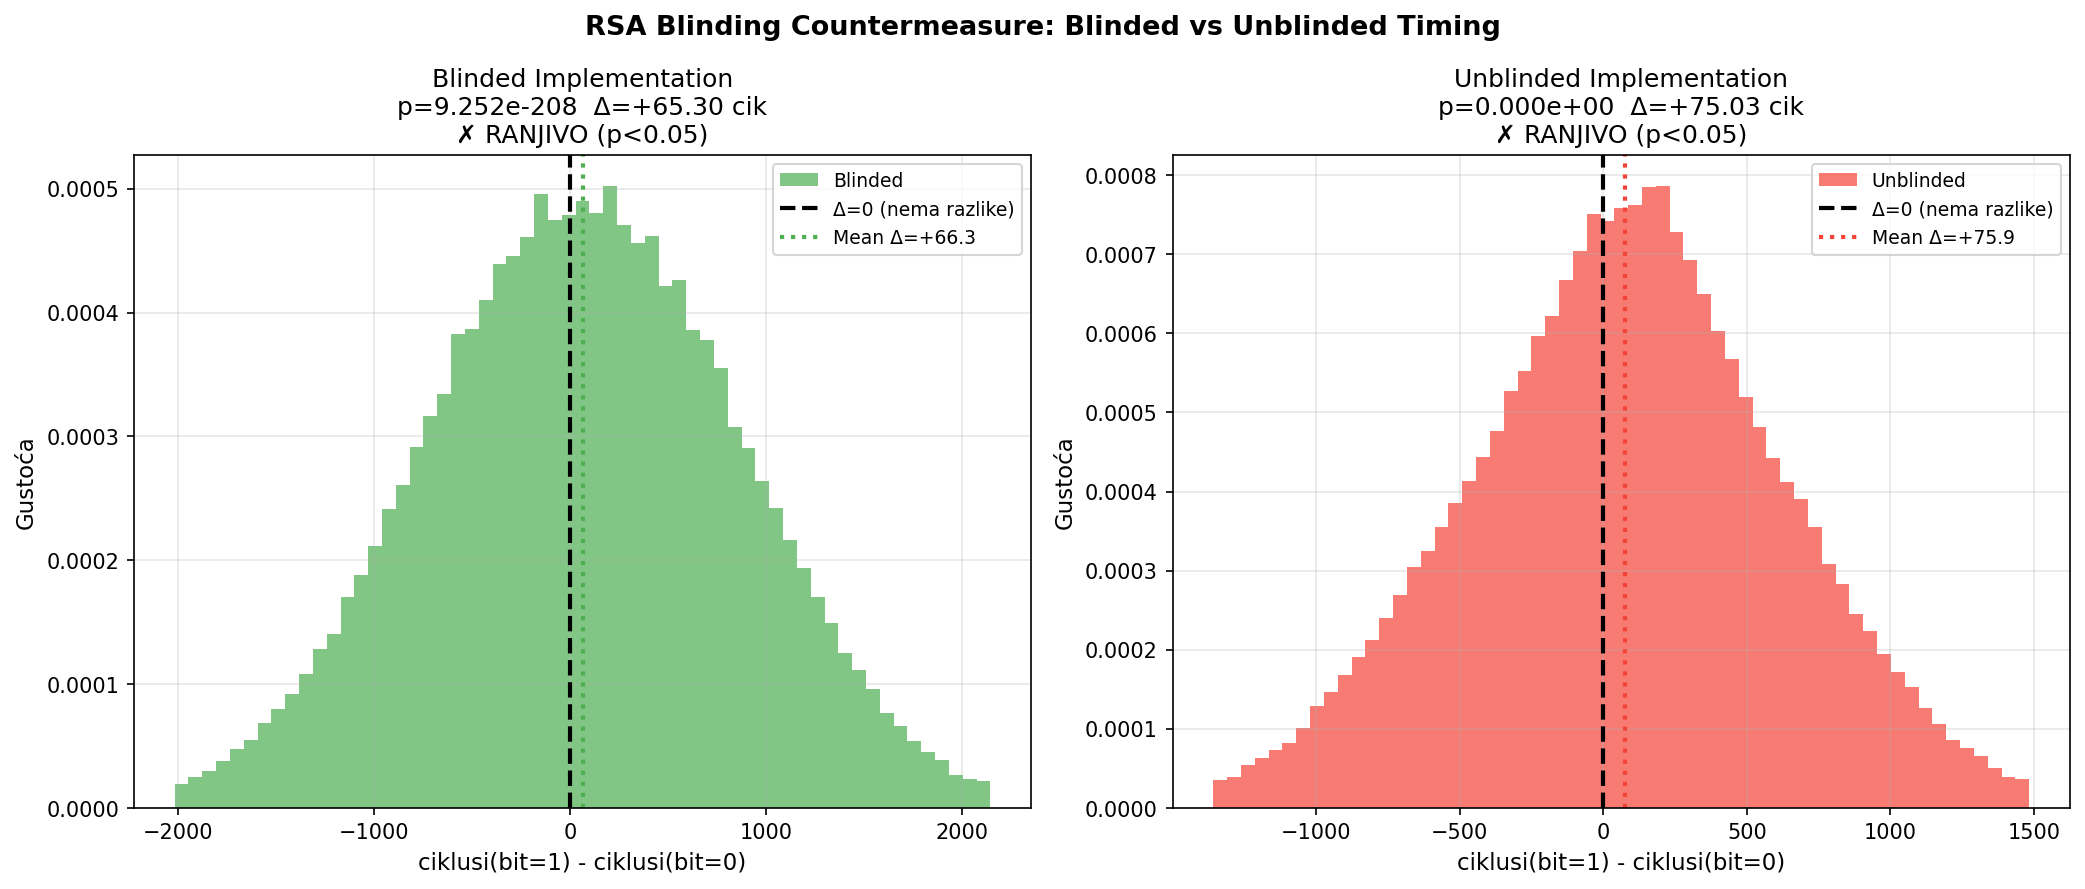
\includegraphics[width=\textwidth]{plot_blinding.png}
\caption{Evaluacija RSA blindinga kao kontramjere: distribucija parnih timing razlika za blinded (zelena) i unblinded (crvena) varijantu}
\label{fig:blinding}
\end{figure}

Blinding smanjuje timing razliku sa +75{,}03 na +65{,}30 ciklusa (redukcija od približno 13\%) i Cohen-ov $d$ sa 0{,}125 na 0{,}098. Međutim, signal i dalje ostaje statistički visoko značajan ($p = 9{,}3 \times 10^{-208}$), što znači da blinding ne eliminiše vremensko curenje.

Smanjenje signala od 13\% ima dva moguća objašnjenja. Prvo, instrukcija \texttt{MULQ} na testiranom procesoru možda ima male operand-zavisne timing varijacije koje blinding djelomično maskira promjenom ulaznih operanada. Drugo, blinded varijanta ima duže ukupno trajanje ($\approx 11\,740$ naspram $\approx 8\,770$ ciklusa za unblinded) jer koristi veće brojeve, što povećava apsolutnu varijansu i time razvodnjava relativnu veličinu signala. Razdvajanje ovih dviju hipoteza zahtijevalo bi izoliranu analizu latencije \texttt{MULQ}.

\subsection{Analiza: zašto blinding ne eliminiše leak}

Ovaj rezultat nije posljedica implementacijske greške, već fundamentalna posljedica arhitekture napada. U ovoj 64-bitnoj implementaciji, vremensko curenje dolazi od grananja u square-and-multiply algoritmu: za bit=1 izvršava se dodatni poziv \texttt{mulmod()} (grananje), dok se za bit=0 taj poziv preskače.

Blinding mijenja bazu (ulaz u množenje), ali ne mijenja eksponent $d$. Obrazac grananja \texttt{if ((exp >> i) \& 1)} ostaje identičan bez obzira na to koja je baza korištena. Dodatno, 64-bitna \texttt{MULQ} instrukcija na x86 izvršava množenje u konstantnom vremenu za sve operande, pa blinding ne može maskirati operand-zavisne varijacije jer ih na ovoj širini operanda praktično nema.

U realnom RSA s big-number aritmetikom (biblioteke poput GMP ili OpenSSL), situacija je suštinski drugačija. Višeprecizno množenje velikih brojeva (npr. 2048-bitnih) nije constant-time jer trajanje zavisi od efektivne veličine operanada i broja propagacija carry bita. U tom scenariju blinding randomizira međuvrijednosti i maskira operand-zavisni timing signal, čineći ga efikasnom kontramjerom \cite{brumley2003}.

Ovaj eksperiment demonstrira važnu razliku između dvije različite vrste vremenskog curenja:

\begin{description}
\item[Branch-zavisni leak] (korišten u ovim eksperimentima): Trajanje zavisi od kontrolnog toka, tj. od toga koji se put kroz kod izvršava. Blinding ne pomaže jer ne mijenja kontrolni tok.
\item[Operand-zavisni leak] (prisutan u realnom RSA s aritmetikom velikih brojeva): Trajanje zavisi od numeričke veličine operanada. Blinding pomaže jer nasumično bira operande čime onemogućuje napadaču da poveže trajanje s poznatim ulazom.
\end{description}

% ---------------------------------------------------------------

\section{Eksperiment 7: Flush+Reload cache napad}
\label{sec:fr_exp}

\subsection{Motivacija}

Eksperimenti 1--6 demonstriraju timing side-channel napade koji mjere ukupno trajanje kriptografske operacije. Međutim, postoji fundamentalno drugačija klasa napada koja umjesto ukupnog trajanja prati prisutnost specifičnih funkcija u CPU cache memoriji i njihovo vrijeme pristupa. Flush+Reload napad \cite{yarom2014} koristi fizički dijeljenu Last Level Cache (LLC) između procesa i može detektovati izvršavanje pojedinačnih funkcija iz dijeljene biblioteke bez mjerenja ukupnog trajanja.
\\

Ova klasa napada ima nekoliko praktičnih prednosti pred timing napadom. Napad funkcioniše čak i kada je žrtva na drugom CPU jezgru (bez dijeljenog L1/L2 cache-a), radi u prisustvu jačeg šuma (mrežna aktivnost, virtualizacija) jer signal ne zavisi od ukupnog trajanja operacije, i cilja specifičnu funkciju umjesto globalnog vremenskog signala.

Razlika od 341{,}5 ciklusa između cache hit-a i miss-a daleko je jača od vremenskog signala iz prethodnih eksperimenata (76 ciklusa), što čini klasifikaciju trivijalno lakom bez statističkog usrednjavanja.

\subsection{Princip Flush+Reload napada}

Princip Flush+Reload napada opisan je u sekciji \ref{sec:cache_attacks}: napadač u ciklusu izbacuje cache liniju ciljane funkcije (\texttt{clflush}), čeka da žrtva potencijalno izvrši operaciju, a potom mjeri reload latenciju. Kratka latencija ($\approx 340$ ciklusa) ukazuje na cache hit i zaključuje da je bit eksponenta jednak 1; duga latencija ($\approx 681$ ciklusa) ukazuje na cache miss i zaključuje da je bit jednak 0. Na x86 arhitekturi, svi procesi koji mapiraju isti \texttt{.so} fajl dobijaju iste fizičke okvire stranica, što je preduvjet za dijeljenu LLC cache memoriju.

\subsection{Implementacija}

Implementacijski detalji (dijeljeni RSA kod, pribavljanje adrese putem \texttt{dlsym()}, CPU pinning žrtve na zasebni fizički core i kalibracija praga) opisani su u sekciji~\ref{sec:fr_impl}. Žrtva između dekriptacija pauzira $50\,\mu\mathrm{s}$\footnote{Pri trajanju jedne dekriptacije od $\approx 4{,}2\,\mu\mathrm{s}$, aktivna frakcija iznosi $4{,}2/(4{,}2+50)\approx 7{,}7\,\%$ ukupnog vremena.}, što daje jasne granice između operacija i odgovara tipičnom primjeru kriptografskog servera s umjerenim opterećenjem.

\subsection{Rezultati}

\begin{table}[H]
\centering
\caption{Rezultati Flush+Reload napada na \texttt{rsa\_multiply\_step()}}
\label{tab:flush_reload}
\begin{tabular}{ll}
\toprule
\textbf{Metrika} & \textbf{Vrijednost} \\
\midrule
Broj observacija           & 100\,000 \\
Cache hitovi (bit=1)       & 45\,095 (45{,}1\%) \\
Cache miss-ovi (bit=0)     & 54\,905 (54{,}9\%) \\
Mean reload latencija (hit)  & 339{,}9 ciklusa \\
Mean reload latencija (miss) & 681{,}4 ciklusa \\
Razlika (miss $-$ hit)    & \textbf{341{,}5 ciklusa} \\
\bottomrule
\end{tabular}
\end{table}

\begin{figure}[H]
\centering
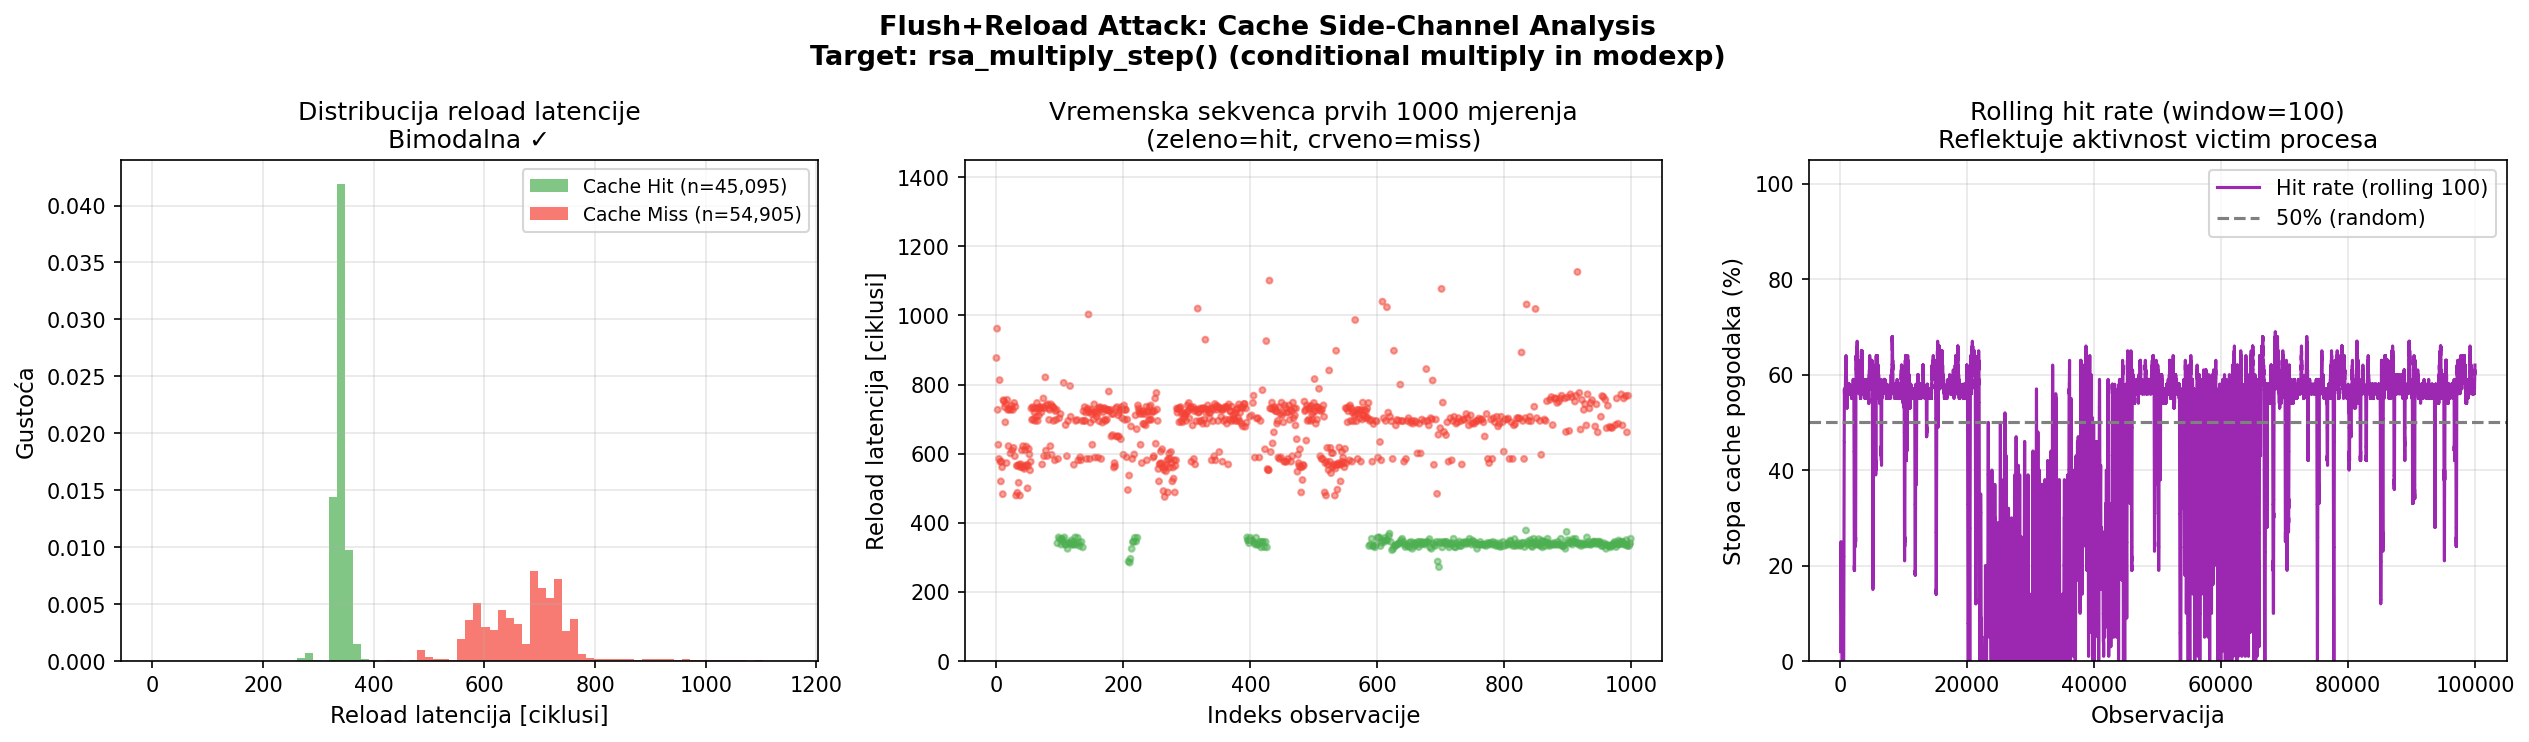
\includegraphics[width=\textwidth]{plot_flush_reload.png}
\caption{Histogram reload latencija: bimodalna distribucija, vremenska sekvenca mjerenja i rolling hit rate}
\label{fig:flush_reload}
\end{figure}

Slika \ref{fig:flush_reload} prikazuje bimodalnu distribuciju reload latencija sa dva jasno odvojena pika. Cache hit (žrtva je pozvala \texttt{rsa\_multiply\_step()}, što znači da je bit eksponenta jednak 1) daje prosječnu latenciju od 339{,}9 ciklusa, što odgovara latenciji pristupa LLC-u. Cache miss (funkcija nije bila pozvana) daje 681{,}4 ciklusa, što odgovara latenciji pristupa glavnoj memoriji (DRAM). Separacija od 341{,}5 ciklusa između cache hit-a i miss-a priblizno je 4{,}5 puta veća od timing signala iz prethodnih eksperimenata.

Udio cache hitova od 45{,}1\% je veći od naivne procjene zasnovane na aktivnoj frakciji i udjelu jediničnih bita ($7{,}7\% \times 72\% \approx 5{,}5\%$). Ova razlika objašnjava se perzistencijom podataka u LLC-u: kada žrtva pozove \texttt{rsa\_multiply\_step()}, odgovarajuća cache linija ostaje u LLC-u znatno duže od jednog intervala. Budući da se unutar jedne dekriptacije funkcija poziva za svaki od $\approx 34$ bita koji su jednaki 1, cache linija je prisutna u LLC-u tokom značajnog dijela aktivnog perioda žrtve, i napadač može detektovati hit čak i ako je konkretni poziv završio ranije.

\subsection{Poređenje s timing napadom}

Flush+Reload i timing napad ciljaju istu osnovnu ranjivost (uslovno grananje u square-and-multiply), ali koriste suštinski različite mehanizme detekcije:

\begin{table}[H]
\centering
\caption{Poređenje timing napada i Flush+Reload napada}
\label{tab:attack_comparison}
\begin{tabular}{lll}
\toprule
\textbf{Dimenzija} & \textbf{Timing napad (Eksperimenti 1--4)} & \textbf{Flush+Reload (Eksperiment 7)} \\
\midrule
Signal & $\approx 76$ ciklusa & $\approx 342$ ciklusa \\
Granularnost & Cijela operacija & Pojedinačna funkcija \\
Šum & Visok (OS, cache, TLB) & Nizak (bimodalna distribucija) \\
Mjerenja/bit & $K \geq 2000$ za 100\% & 1 mjerenje (threshold) \\
Dijeljeni resursi & Ništa & Dijeljeni LLC \\
Constant-time zaštita & Eliminiše napad & Eliminiše napad\footnotemark \\
\bottomrule
\end{tabular}
\end{table}

\footnotetext{Za Flush+Reload, zaštita je teoretski izvedena: constant-time implementacija izvršava obje operacije uvijek, pa bi ciljna funkcija bila prisutna u cache-u neovisno o vrijednosti bita. Ovo nije eksperimentalno verificirano u okviru ovog rada, i zahtijeva da obje putanje pristupaju istim cache linijama. Eksperimentalnu verifikaciju ove tvrdnje treba smatrati otvorenim pravcem za buduće istraživanje; u kontekstu ovog rada, zaštitu constant-time implementacije od Flush+Reload napada treba tretirati kao teorijsku pretpostavku, ne empirijsko tvrđenje.}

Najznačajnija razlika je u potrebnom broju mjerenja. Timing napad zahtijeva usrednjavanje $K = 2000$ mjerenja po bitu za postizanje 100\% tačnosti, dok Flush+Reload može klasificirati bit iz jednog jedinog mjerenja zahvaljujući daleko većem signalu (341 naspram 76 ciklusa). S druge strane, Flush+Reload zahtijeva da napadač i žrtva dijele istu fizičku memoriju (isti \texttt{.so} fajl), što ograničava primjenjivost na scenarije s dijeljenim bibliotekama.

Ova Flush+Reload implementacija je kontrolisani dokaz koncepta s namjerno izolovanom ciljnom funkcijom. U stvarnim kriptografskim bibliotekama, razlika između kvadriranja i množenja u funkcijama postojala je prirodno. 
Upravo takve prirodne separacije su motivisale Yarom i Falkner \cite{yarom2014} da demonstriraju ovaj napad i time potaknu prelazak na konstantne vremenske implementacije u modernim kriptografskim bibliotekama.

% ---------------------------------------------------------------
\section{Diskusija}

\subsection{Interpretacija Cohen-ovog d = 0{,}134}

Mali Cohen-ov $d$ ne umanjuje značaj nalaza. Ova vrijednost kvantificira fizičku veličinu efekta: signal od 76 ciklusa u šumu od $\sigma \approx 567$ ciklusa daje odnos signala i šuma (SNR) od 0{,}134 po pojedinačnom uzorku. Ovakav odnos je tipičan za timing napade na modernom procesoru, gdje su izvori šuma znatni (cache miss-ovi, pogrešna predviđanja grananja, preempcije operativnog sistema).

Ono što čini ovaj signal iskoristivim za napad je njegova konzistentnost i determinističnost. Signal se pojavljuje identično na medijani, P25 i P75 (Eksperiment 1), na svih 64 pozicija bita (Eksperiment 4), i pri različitim nivoima optimizacije (Eksperiment 5). Budući da je signal konzistentan a šum slučajan, usrednjavanje ga pouzdano "izvlači": $K = 2000$ uzoraka je dovoljno za 100\% tačnost klasifikacije (Eksperiment 2).


\subsection{Praktična cijena napada na realni RSA}

Eksperiment koristi 64-bitni privatni eksponent radi brzog izvođenja, ali mehanizam je identičan za realni RSA s 2048-bitnim ključem jer se svaki bit napada nezavisno istom tehnikom. Napad se konceptualno skalira linearno jer se informacije o bitovima privatnog eksponenta izdvajaju iterativno korištenjem iste metodologije mjerenja: za potpunu rekonstrukciju 2048-bitnog ključa potrebno je $2048 \times 5000 \times 2 \approx 20{,}5$ miliona mjerenja (5000 mjerenja po bitu, dva mjerenja po paru).

Pri prosječnom trajanju jedne 2048-bitne modularne eksponencijacije od $\approx 1$--$5$ ms (realistično za softversku aritmetiku velikih brojeva na standardnom savremenom procesoru), ukupno vrijeme napada iznosi od $\approx 5{,}7$ sati do $\approx 28{,}5$ sati. Sa CRT (\textit{Chinese Remainder Theorem} -- Kineski teorem o ostacima) optimizacijom koja ubrzava RSA dekriptovanje za faktor $\approx 4\times$, procjena se spušta na $\approx 1{,}4$--$7$ sati. Ovo ilustruje da timing napad nije isključivo teorijski, već je praktično izvodljiv u razumnom vremenskom okviru, pogotovo s obzirom na to da se napad može paralelizovati za pozicije bita.

U mrežnom scenariju svako mjerenje uvodi $\approx 0{,}1$--$1$ ms dodatne latencije, pa bi 20 miliona mjerenja trajalo od nekoliko sati do nekoliko dana, zavisno od mrežne udaljenosti i metode pojačavanja signala \cite{brumley2003}.

\subsection{Primjenjivost na moderne RSA biblioteke}

Napad demonstriran u ovom radu zasniva se na klasičnoj square-and-multiply implementaciji modularne eksponencijacije koja koristi eksplicitno grananje zavisno od vrijednosti bitova privatnog eksponenta. Savremene kriptografske biblioteke, poput \textit{OpenSSL}-a i \textit{libgcrypt}-a, uglavnom implementiraju različite zaštitne mehanizme kako bi se smanjilo curenje vremenskih informacija, čime se značajno otežava izvođenje klasičnih timing napada.

Ipak, zaštita od timing napada ne zavisi isključivo od algoritma, već i od načina implementacije aritmetike velikih brojeva. Implementacije koje ne koriste operacije konstantnog vremena nad operandima i dalje mogu otkrivati informacije kroz suptilne razlike u vremenu izvršavanja. Zbog toga manje poznate, prilagođene ili nestandardne kriptografske biblioteke mogu ostati ranjive čak i kada koriste moderne algoritamske optimizacije.


